\chapterimage{orange2.jpg}
\chapterspaceabove{6.75cm} 
\chapterspacebelow{7.25cm} 
\chapter{Random Variable and Discrete Distribution}
Random variables are fundamental concepts in probability theory, describing 
quantities whose values result from random phenomena. This chapter delves into 
discrete random variables and their distributions, exploring how they are used to modeling 
and analyze situations where outcomes are countable.

\begin{itemize}
    \item \textbf{Definition of Random Variables:} We start by defining random 
    variables and discussing their basic properties, including how they function 
    within the framework of probability theory.
    
    \item \textbf{Expectation and Variance:} This section covers the computation 
    and implications of expectation and variance, which describe the average 
    outcome of a random variable and the spread of its outcomes, respectively.
    
    \item \textbf{Common Discrete Distributions:} We explore well-known 
    distributions such as the Binomial and Poisson distributions, which are 
    essential for modeling many real-world processes.
    
    \item \textbf{Other Discrete Distributions:} Additional discrete distributions 
    are discussed, providing insights into more specialized or less commonly 
    encountered models.
    
    \item \textbf{Properties of Random Variables, PDF, and CDF:} The chapter 
    concludes with an examination of the mathematical properties of random 
    variables, including their probability distribution functions and cumulative 
    distribution functions.
\end{itemize}

Each section includes exercises that challenge the reader to apply theoretical 
concepts to practical problems, reinforcing learning and enhancing understanding 
of random variables and discrete distributions.

\section{Random Variable}
We First define random variables and discuss their basic properties, including how they function within the framework of probability theory.
In a short word, a random variable is a functional relation between the possible outcomes of a random experiment
and the probability of each outcome. It assigns a real number to each outcome in the sample space of a random experiment. Though we call it a \textbf{variable}, it is actually a function.
\begin{definition}[Random Variable]
    A \textbf{random variable} is a function \( X: S \rightarrow \mathbb{R} \) 
    where \( S \) is the sample space of a random experiment. This function 
    assigns a real number to each outcome in the sample space \( S \). 
    
    The mapping \( X \) is defined such that for any outcome \( \omega \) 
    in the sample space \( S \), \( X(\omega) \) specifies a real number 
    that represents a possible value of the random variable in the context 
    of the experiment. This allows the random variable to quantify 
    the outcomes of the experiment in numerical terms.
\end{definition}

A random variable \( X \) can be thought of as a rule or a function that assigns 
a specific number to each possible outcome of a random experiment. The sample 
space \( S \) includes all possible outcomes of this experiment. For each 
outcome \( \omega \) in \( S \), the random variable \( X \) gives a number 
\( X(\omega) \). This number is not random; it is fixed for each outcome 
\( \omega \).

This mapping can be a little abstract, but in a short word, random variable is a way to represent 
the outcomes of a random experiment in numerical terms, which make it easier to analyze and make predictions about the outcomes of the experiment.

Here are some practical examples of random variables.
\begin{example}[Tossing a Coin]
    Consider a random experiment where we toss a fair coin. Define the sample space 
    \( S = \{\text{Heads}, \text{Tails}\} \). Let \( X \) be a random variable that 
    assigns \( 1 \) if the outcome is Heads and \( 0 \) if the outcome is Tails. Thus, 
    \( X(\text{Heads}) = 1 \) and \( X(\text{Tails}) = 0 \). Here, \( X \) is used to 
    numerically represent the outcomes of a coin toss.
    \end{example}
    
    \begin{example}[Daily Temperature]
    Consider measuring the high temperature in a particular city on a given day. 
    Define \( X \) to be the random variable representing the high temperature 
    recorded on that day. If the thermometer reads 20 degrees Celsius, then 
    \( X(\omega) = 20 \) where \( \omega \) is the outcome of that day's temperature 
    measurement. This example shows how random variables can be used to model 
    quantitative data in environmental studies.
    \end{example}
    
    \begin{example}[Number of Customers]
    Suppose a shop wants to analyze the number of customers that enter the store 
    each day. Let \( X \) be a random variable representing the total number of 
    customers on any given day. If 250 customers enter the shop on a particular day, 
    then \( X(\omega) = 250 \), indicating the count of customers as the outcome 
    of the random variable.
    \end{example}
    
    \begin{example}[Sum of Dice Rolls]
    Consider rolling two six-sided dice and let \( X \) be the random variable 
    representing the sum of the numbers on the two dice. The sample space \( S \) 
    consists of all pairs of numbers from 1 to 6 for each die. For an outcome 
    \( \omega = (3, 4) \), where the first die shows 3 and the second die shows 4, 
    the random variable \( X \) would give \( X(\omega) = 3 + 4 = 7 \). This is a 
    classical example used in probability theory to introduce the concept of sum 
    distributions.
    \end{example}

The purpose of this mapping is to numerically represent the results of 
random processes, allowing us to apply mathematical tools to analyze 
and make predictions about these processes. The mapping defined by \( X \) 
is deterministic within the experiment context—once the outcome \( \omega \) 
is realized, the value \( X(\omega) \) is definitively known. 

Another question is that, are random variable always discrete? The answer is no. Random variables can be either discrete or continuous, depending on the nature of the outcomes they represent. Discrete random variables are those that take on a finite or countably infinite number of distinct values, while continuous random variables can take on any value within a specified range. In this chapter, we focus on discrete random variables and their distributions, 
which are essential for modeling and analyzing situations where outcomes are countable.
We have seen many examples of discrete random variables in the previous examples. 
And this chapter involves indeed only discrete random variables. Still, we provide an example of continuous random variables for completeness.

\begin{example}[Height of Students]
Let \( X \) be a continuous random variable representing the height (in centimeters) 
of students in a high school. The exact height of a student can be any value within 
a range, making \( X \) a continuous random variable. The probability of \( X \) 
taking any specific value is zero, but probabilities can be assigned to ranges of 
values (e.g., the probability that a student's height is between 160 cm and 170 cm).
\end{example}

\begin{example}[Time Required to Complete a Task]
Suppose \( T \) represents the time (in hours) required to complete a specific task. 
\( T \) is a continuous random variable because the completion time can be any 
real number within a certain interval, depending on various factors like speed, 
efficiency, and interruptions.
\end{example}

\begin{example}[Amount of Rainfall]
Let \( R \) be a continuous random variable representing the amount of rainfall 
(in millimeters) received in a city on a given day. Rainfall can be measured as 
any non-negative real number, making \( R \) a perfect example of a continuous 
random variable, where you can find the probability of receiving more than a 
certain amount of rainfall but not the probability of an exact amount.
\end{example}

\begin{example}[Temperature Measurement]
Consider \( \Theta \) as a continuous random variable representing the temperature 
(in degrees Celsius) at noon in a particular location. Temperature is inherently 
continuous as it can take any value within a possible range, and minor variations 
are always possible, making \( \Theta \) continuously variable.
\end{example}

You may have realized that dealing with continuous random variables requires knowledge of calculus and integration.
In this chapter, we focus on discrete random variables, which are easier to work with and provide a solid foundation for understanding more complex probability concepts.
\subsection{Analysis of Random Variables}
The random variable itself seems to be a simple concept, but it is essential in probability theory.
What can we do with random variables? We can analyze them in various ways to understand the underlying probability distributions and make predictions about the outcomes of random processes.
We have seen many examples of analyzing random events and the probability of events in the previous chapters.
In those cases, we found probability given a specific event or a set of events.
With random variable, we can model the pattern of probability distribution of the outcomes of the random process
in all cases.

Here is a simple example of analyzing a random variable in a given situation.
\begin{example}[Tossing Three Coins]
    Suppose our experiment consists of tossing three fair coins. If we let \( Y \) denote the number of heads that appear, then \( Y \) is a random variable taking on one of the values 0, 1, 2, and 3 with respective probabilities:

\begin{itemize}
    \item \( P(Y = 0) = P(\text{T, T, T}) = \frac{1}{8} \)
    \item \( P(Y = 1) = P(\text{T, T, H}) + P(\text{T, H, T}) + P(\text{H, T, T}) = 3 \times \frac{1}{8} = \frac{3}{8} \)
    \item \( P(Y = 2) = P(\text{T, H, H}) + P(\text{H, T, H}) + P(\text{H, H, T}) = 3 \times \frac{1}{8} = \frac{3}{8} \)
    \item \( P(Y = 3) = P(\text{H, H, H}) = \frac{1}{8} \)
\end{itemize}

Since \( Y \) must take on one of the values 0 through 3, we must have:
\[ 
1 = P\left( \bigcup_{i=0}^{3} \{Y = i\} \right) = \sum_{i=0}^{3} P(Y = i)
\]
which, of course, is in accord with the preceding probabilities, because all these
cases are disjoint and combine to cover all possibilities.
\end{example}

With random variable, we can model more complex situations and analyze the probability distribution of the outcomes.
Here is a more complex example of analyzing a random variable in a given situation.
\begin{example}[Coin Flipping]
    Consider an experiment where we flip a coin that has a probability \( p \) of 
coming up heads. We continue flipping the coin until either a head appears or 
we have flipped the coin \( n \) times. Let \( X \) denote the number of times 
the coin is flipped. Then, \( X \) is a random variable that can take on values 
from 1 to \( n \), where each value corresponds to the number of flips made.

The probabilities for each outcome are calculated as follows:
\begin{itemize}
    \item \( P(X = 1) = p \) (The probability of getting heads on the first flip)
    \item \( P(X = 2) = (1 - p) p \) (The probability of getting tails first, then heads)
    \item \( P(X = 3) = (1 - p)^2 p \) (The probability of getting tails twice, then heads)
    \item \dots
    \item \( P(X = n - 1) = (1 - p)^{n-2} p \) (The probability of getting tails \( n-2 \) times, then heads)
    \item \( P(X = n) = (1 - p)^{n-1} \) (The probability of getting tails \( n-1 \) times, if \( n \) flips are made and no heads appear)
\end{itemize}

As a verification, the sum of all probabilities must equal 1:
\[
\sum_{i=1}^{n} P(X = i) = p \sum_{i=1}^{n-1} (1 - p)^{i-1} + (1 - p)^{n-1}
\]
\[
= p \frac{1 - (1 - p)^{n-1}}{1 - (1 - p)} + (1 - p)^{n-1}
\]
\[
= p \left(\frac{1 - (1 - p)^{n-1}}{p}\right) + (1 - p)^{n-1}
\]
\[
= 1 - (1 - p)^{n-1} + (1 - p)^{n-1}
\]
\[
= 1
\]

This confirms that the calculated probabilities are correct and all possibilities 
have been accounted for.
\end{example}

\subsection{Discrete Random Variables and Discrete Distributions}
Now we shall give a strict definition to distribution of discrete random variables, which we 
also call discrete probability distribution.
\begin{definition}[Discrete Probability Distribution]
    A \textbf{discrete probability distribution} is a function that assigns 
    probabilities to each possible value of a discrete random variable. 
    This function specifies the probability of each possible outcome of the 
    random variable, allowing us to analyze the likelihood of different values 
    occurring.
    A discrete probability distribution is characterized by a probability mass function \( p \) which assigns a probability \( p(x) \) to each possible value \( x \) of the discrete random variable \( X \). The function \( p \) satisfies the following conditions:
\begin{itemize}
    \item \( p(x) \geq 0 \) for all \( x \) in the domain of \( X \),
    \item \( \sum_{x} p(x) = 1 \), where the sum extends over all possible values of \( X \).
\end{itemize}

The distribution is \textit{discrete} because the sum involves a countable number of terms, and the random variable \( X \) takes on countable, typically finite, distinct values.
\end{definition}

Probability distributions are modeled using probability functions. Here we also give 
a strict definition to these functions.

\begin{definition}[Probability Measure of Random Variable]
    The probability that \( X \) takes on a specific value \( x \) from \( \mathbb{R} \) is given by:
    \[ P(X = x) = P(\{\omega \in S \mid X(\omega) = x\}) \]
    This expression evaluates the measure of the set of all outcomes \( \omega \) in \( S \) for which the value of the random variable \( X \) equals \( x \).

\end{definition}
Probability measure is a measure of the likelihood of a specific value of a random variable.
While it is not a probability distribution or function, but just an independent measure 
of the likelihood of a specific value of a random variable.

\begin{definition}[Probability Function of Random Variable]
    For a discrete random variable \( X \) defined on a sample space \( S \), the probability function \( P \) can be described by a mapping:
    \[
    P: \mathcal{P}(S) \to [0, 1]
    \]
    where \( \mathcal{P}(S) \) is the power set of \( S \), representing all possible subsets of \( S \). For each event \( A \subset S \), the probability function is defined as:
    \[
    P(A) = \sum_{\omega \in A} P(\{\omega\})
    \]
    assuming \( P(\{\omega\}) \) specifies the probability of the elementary event \( \{\omega\} \).
    
    In the context of a random variable, the mapping can also be represented specifically for the outcomes of \( X \) as:
    \[
    P_X: \mathbb{R} \to [0, 1]
    \]
    with:
    \[
    P_X(x) = P(X = x) = P(\{\omega \in S \mid X(\omega) = x\})
    \]
    This means the probability that some elements $\omega$ of the sample space $S$, where $\omega$ that satisfies $X(\omega)=x$ by the random variable $X$ to some real number $x$ (in the case of discrete distribution, $x\in \Z$).
    
    This function \( P_X \) gives the probability that \( X \) takes any particular value \( x \).    
\end{definition}
\begin{remark}
    Note that, the probability function in this context is called \textbf{Probability Density function (PDF)}. We will also discuss the other probability function called \textbf{Cumulative Density Function (CDF)} and discuss their relation. Their properties will also be discussed at the end of this chapter.
\end{remark}
We illustrate with an example of fair dice rolling.
\begin{example}[Rolling a Fair Six-Sided Die]
    Let \( X \) be the random variable representing the outcome of rolling a fair six-sided die. The possible outcomes for \( X \) are 1, 2, 3, 4, 5, and 6. Since the die is fair, the probability of each outcome is equal. Thus, the probability function for \( X \) is given by:
    \[
    P(X = x) = \frac{1}{6}, \text{ for } x = 1, 2, 3, 4, 5, 6
    \]
    and \( P(X = x) = 0 \) for all other values of \( x \). We are not plottig it here for clarity, but doesn't mean the function is not defined for other possible value of $X = x\in \{\Z^+ - \{1, 2, 3, 4, 5, 6\}\}$.

\begin{center}
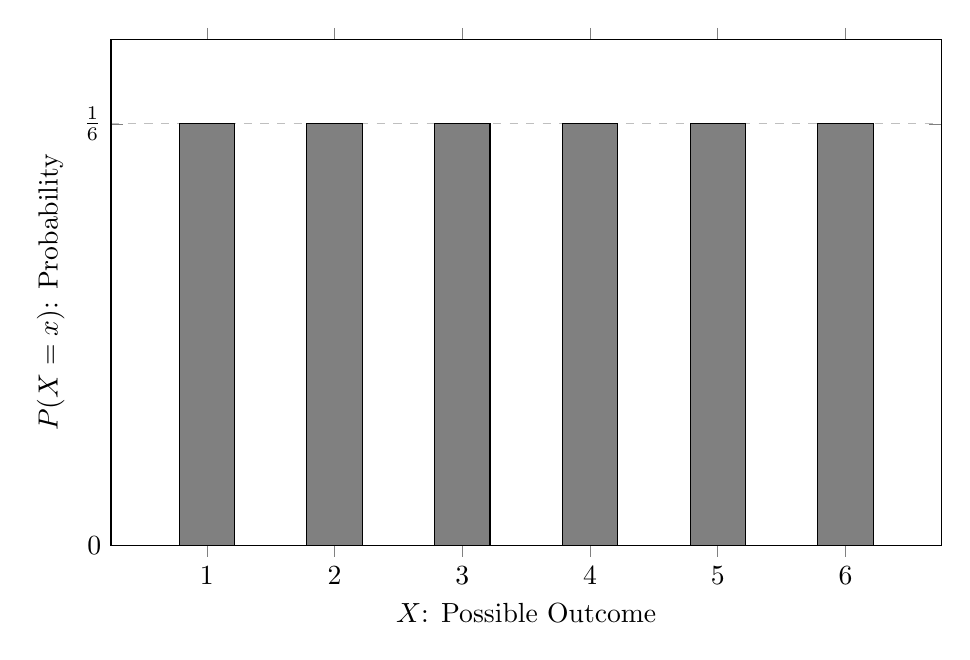
\begin{tikzpicture}
\begin{axis}[
    ybar, 
    bar width=20pt,
    width=\textwidth,
    height=8cm,
    xlabel={$X$: Possible Outcome},
    ylabel={$P(X=x)$: Probability},
    symbolic x coords={1,2,3,4,5,6},
    xtick=data,
    ymin=0, ymax=0.20, % Adjust the maximum y-value appropriately
    ytick={0, 0.1667}, % Use decimal equivalent of 1/6
    yticklabels={0, $\frac{1}{6}$}, % You can still use fractions in labels for clarity
    nodes near coords,
    nodes near coords align={vertical},
    enlarge x limits=0.15,
    ymajorgrids=true,
    grid style=dashed,
]

\addplot[fill=gray, nodes near coords=] coordinates {
    (1,0.1667) (2,0.1667) (3,0.1667) (4,0.1667) (5,0.1667) (6,0.1667)
};
\end{axis}
\end{tikzpicture}
\end{center}

    This plot shows the uniform probability distribution for each outcome of rolling the die.
\end{example}

It is noticeable that for each possible $x$, $P(X=x)$ has the same value $\frac{1}{6}$. 
Actually, this distribution is categorized as a kind of special, but most basic discrete distribution, called \textbf{Uniform Discrete Distribution}.

We have been using the terms discrete distribution and discrete probability function. They are very close to each other, while we need to differentiate them in many aspects.
A probability function and a probability distribution are related but distinct concepts in probability theory. The key difference lies in their scope and representation.

A probability function specifies the probability of each individual outcome or value of a random variable. It provides a point-wise description of the likelihood of different outcomes.

On the other hand, a probability distribution is a more comprehensive concept that encompasses the collective behavior of a random variable. It describes the overall probabilistic properties of the random variable, often by specifying the probabilities associated with different ranges or sets of outcomes.
\subsection{Exercises}

\section{Expectation and Variance}
Since we have defined probability distribution and probability density function. We can now investigate more aspects of the function. Recall that in calculus, the average value of a continuous function $f(x)$ defined on the interval $[a, b]$ is given by the formula:
\begin{equation}
\text{Average Value} = \frac{1}{b - a} \int_{a}^{b} f(x) \, dx
\end{equation}
where:
\begin{itemize}
    \item $\int_{a}^{b} f(x) \, dx$ represents the definite integral of the function $f(x)$ over the interval $[a, b]$, which calculates the accumulated area or value of the function within that interval.
    \item $b - a$ represents the length of the interval.
    \item The integral is divided by the interval length to obtain the average value or average level of the function over that interval.
\end{itemize}
For a normal discrete function, the integral is replaced by a summation:
\begin{equation}\label{dissum}
\text{Average Value} = \frac{1}{n} \sum_{i=1}^{n} f(x_i)
\end{equation}

where $n$ is the number of discrete points, and $x_i$ are the discrete values at which the function is evaluated.

\subsection{Expectation of Discrete Random Variable}
Of course we know that discrete random distribution are modeled by discrete function. But things are slightly different here, since when we deal with a normal discrete function, it is implied that we are treated each value equally, if you take that $\frac{1}{n}$ as the possibility of each value appearing. While for discrete distribution this is a different story, because we only see such cases when we have a uniform distribution like rolling a dice. To generalize this expression, we can replace the uniform probability with a the probability that each value $x_i$ occur, which is actually a weighted average. Now we can define expectation of discrete random variable.
\begin{definition}[Expectation of Discrete Random Variable]
The expectation $E$ of a discrete random variable $X$ is the weighted average of the possible values that $x\in \text{range}(X)$ can be taken.
\begin{equation}
E[X] = \sum_{xp(x) > 0} xp(x)
\end{equation}
Where $P(x)$ is derived form the uniform probability $\frac{1}{n}$, and $x$ is derived from $f(x_i)$ in equation \ref*{dissum}.
\end{definition}

\begin{example}[Fair Dice]
    When we roll a clear dice, since each side has a chance of $\frac{1}{6}$.
    Let $\text{range}(X) = \{1,2,3,4,5,6\}$We have 
    \[
    E[X] = 1\left(\frac16\right)+2\left(\frac16\right)+3\left(\frac16\right)+4\left(\frac16\right)+5\left(\frac16\right)+6\left(\frac16\right)=\frac72
    \]
\end{example}

\begin{example}
    A school class of 120 students is driven in 3 buses to a symphonic performance. There are 36 students in one of the buses, 40 in another, and 44 in the third bus. When the buses arrive, one of the 120 students is randomly chosen. Let $X$ denote the number of students on the bus of that randomly chosen student, and find $E[X]$.
    \begin{solution}
        Since the randomly chosen student is equally likely to be any of the 120 students, it follows that
\[
P(X = 36) = \frac{36}{120}, \quad P(X = 40) = \frac{40}{120}, \quad P(X = 44) = \frac{44}{120}
\]
Hence,
\[
E[X] = 36 \left(\frac{3}{10}\right) + 40 \left(\frac{1}{3}\right) + 44 \left(\frac{11}{30}\right) = \frac{1208}{30} \approx 40.2667
\]
    \end{solution}
\end{example}

\subsection{Expectation of Function and Linearity}
Now suppose we want to transform the random variable $X$, for example, apply some function $g(X)$ to change the random variable.
How can we get the composed expectation after transformation? Well, don't be scared, remember that distribution function can be used to calculate $P(g[X])$, and we know the value pf $g[X]$. By the definition, we can calculate $E[g(x)]$.

\begin{example}
    Let $X$ denote a random variable that takes on any of the values $-1$, $0$, and $1$ with respective probabilities
\[
P(X = -1) = 0.2, \quad P(X = 0) = 0.5, \quad P(X = 1) = 0.3
\]
Compute $E[X^2]$.
\begin{solution}
    Let $Y = X^2$. Then the probability mass function of $Y$ is given by
\[
P(Y = 1) = P(X = -1) + P(X = 1) = 0.5, \quad P(Y = 0) = P(X = 0) = 0.5
\]
Hence,
\[
E[X^2] = E[Y] = 1(0.5) + 0(0.5) = 0.5
\]
\begin{remark}
Note that
\[
0.5 = E[X^2] \neq (E[X])^2 = 0.01.
\]
\end{remark}

\end{solution}
\end{example}

However, we can notice that  we can obtain the same result by 
$(-1)^{2}(0.2)\:+\:0^{2}(0.5)\:+\:1^{2}(0.3)$, it seems that we don't have to calculate $P(Y=1)$. This is because $g(X) = g(x)$ when $X = x$, so $E[g(X)]$ is the weighted average of $g(x)$ that $X=x$.
\begin{proposition}
    If $X$ is a discrete random variable that takes on one of the values $x_i,i\geq1$, with
respective probabilities $p(x_i)$, then, for any real-valued function g,
$$E[g(X)]=\sum g(x_i)p(x_i)$$
\end{proposition}
\begin{proof}
Consider a discrete random variable \(X\) taking values \(x_i\) with probability \(p(x_i)\) and a function \(g\) applied to \(X\). Assume \(g(X)\) takes distinct values \(y_j\), \(j \geq 1\). By grouping all the \(x_i\) for which \(g(x_i) = y_j\), the expectation \(E[g(X)]\) can be calculated as follows:
\begin{align*}
E[g(X)] &= \sum_i g(x_i)p(x_i) \\
&= \sum_j \sum_{\{i : g(x_i) = y_j\}} g(x_i)p(x_i) \\
&= \sum_j y_j \sum_{\{i : g(x_i) = y_j\}} p(x_i) \\
&= \sum_j y_j P\{g(X) = y_j\} \\
&= E[g(X)]
\end{align*}
This calculation confirms that the expectation of \(g(X)\) is the sum of the products of each value \(g(x_i)\) takes and the probability of \(x_i\), grouped by the unique values \(y_j\) that \(g\) maps to.
\end{proof}

This brings us to a seemingly conclusion to calculate the expectation of linear combination of random variables.
\begin{corollary}
    A simple logical consequence of Proposition 4.1 is as follows. If \(a\) and \(b\) are constants, then
\[ E[aX + b] = aE[X] + b \]
\end{corollary}
\begin{proof}
    Starting with the linearity of expectation:
\[
E[aX + b] = \sum_{x:p(x)>0} (ax + b)p(x)
\]
This can be rewritten by distributing the expectation:
\[
= a \sum_{x:p(x)>0} xp(x) + b \sum_{x:p(x)>0} p(x)
\]
Recognizing that the sum of the probabilities \( \sum_{x:p(x)>0} p(x) \) equals 1 and \( \sum_{x:p(x)>0} xp(x) \) is \( E[X] \), we obtain:
\[
= aE[X] + b
\]
\end{proof}

We can further generalize this to the linearity of expectation.
\begin{theorem}[Linearity of Expectation Summation]
For any random variables \(X_1, X_2, \ldots, X_n\):
\[
E\left[\sum_{i=1}^n X_i\right] = \sum_{i=1}^n E[X_i].
\]
This property holds regardless of whether the random variables are independent or not.
\end{theorem}
\begin{proof}
    We will prove this by induction on $n$.

    \textbf{Base Case:} For $n = 2$, we need to show that:
    \[
    E[X_1 + X_2] = E[X_1] + E[X_2].
    \]
    By the definition of expectation, we have:
    \begin{align*}
    E[X_1 + X_2] &= \sum_{\omega \in S} (X_1(\omega) + X_2(\omega)) P(\omega) \\
                 &= \sum_{\omega \in S} X_1(\omega) P(\omega) + \sum_{\omega \in S} X_2(\omega) P(\omega) \\
                 &= E[X_1] + E[X_2]
    \end{align*}
    Therefore, the base case holds.

    \textbf{Inductive Step:} Assume the statement holds for some $n = k$, i.e.,
    \[
    E\left[ \sum_{i=1}^k X_i \right] = \sum_{i=1}^k E[X_i].
    \]
    We need to show that the statement holds for $n = k+1$, i.e.,
    \[
    E\left[ \sum_{i=1}^{k+1} X_i \right] = \sum_{i=1}^{k+1} E[X_i].
    \]

    Consider
    \[
    E\left[ \sum_{i=1}^{k+1} X_i \right] = E\left[ \left( \sum_{i=1}^k X_i \right) + X_{k+1} \right].
    \]
    By the linearity of expectation (which states that the expectation of a sum is the sum of the expectations), we have:
    \[
    E\left[ \left( \sum_{i=1}^k X_i \right) + X_{k+1} \right] = E\left[ \sum_{i=1}^k X_i \right] + E[X_{k+1}].
    \]
    Using the inductive hypothesis, we get:
    \[
    E\left[ \sum_{i=1}^k X_i \right] + E[X_{k+1}] = \sum_{i=1}^k E[X_i] + E[X_{k+1}].
    \]
    Therefore,
    \[
    E\left[ \sum_{i=1}^{k+1} X_i \right] = \sum_{i=1}^{k+1} E[X_i].
    \]

    By mathematical induction, the statement holds for all $n \in \mathbb{N}$.
\end{proof}

If you have enough mathematical intuition, you may realized that we can find a similar law for the product of random variables, which is summarized as follows.
But notice that, as we mentioned earlier, expectation is a weighted average based on probability and image of random variable, this rule only holds when all random variables are independent. But how can we define independence of random variable? We can actually duplicate what we have done to define independent event.

\begin{definition}[Independence]
    Random variables \( X_1, X_2, \ldots, X_n \) are said to be \textit{independent} if for any subset of indices \( i_1, i_2, \ldots, i_k \) where \( 1 \leq i_1 < i_2 < \cdots < i_k \leq n \), the joint cumulative distribution function satisfies
    \[
    F_{X_{i_1}, X_{i_2}, \ldots, X_{i_k}}(x_{i_1}, x_{i_2}, \ldots, x_{i_k}) = \prod_{j=1}^k F_{X_{i_j}}(x_{i_j}),
    \]
    for all \( x_{i_1}, x_{i_2}, \ldots, x_{i_k} \in \mathbb{R} \), where \( F_{X_{i_j}}(x) \) denotes the cumulative distribution function of \( X_{i_j} \).

    \textbf{Explanation:} This definition means that the probability distribution of any subset of the random variables can be factored into the product of their individual distributions. In other words, knowing the value of one or more of the variables does not provide any information about the others.
\end{definition}

\begin{definition}[Alternative Definition using Probability]
    Alternatively, random variables \( X_1, X_2, \ldots, X_n \) are independent if for any sets of events \( A_1, A_2, \ldots, A_n \) where \( A_i \) is an event determined by \( X_i \),
    \[
    P(A_1 \cap A_2 \cap \cdots \cap A_n) = P(A_1) \cdot P(A_2) \cdots P(A_n).
    \]

    \textbf{Explanation:} This definition states that the joint probability of all the events occurring simultaneously is equal to the product of their individual probabilities. This implies that the occurrence of one event does not affect the probability of the occurrence of the others.
\end{definition}

Now we can define the linearity of product and prove it by induction.
\begin{theorem}[Linearity of Random Variable Product]
 If all random variables $ X_1, X_2, \ldots, X_k $ are mutually independent, then
    \[
    E\left[ \prod_{i=1}^k X_i \right] = \prod_{i=1}^k E[X_i].
    \]    
\end{theorem}
\begin{proof}
    We will prove this by induction on \( k \).

    \textbf{Base Case:} For \( k = 2 \), we need to show that:
    \[
    E[X_1 \cdot X_2] = E[X_1] \cdot E[X_2].
    \]
    Since \( X_1 \) and \( X_2 \) are independent, we have:
    \[
    E[X_1 \cdot X_2] = E[X_1] \cdot E[X_2].
    \]
    Therefore, the base case holds.

    \textbf{Inductive Step:} Assume the statement holds for some \( k = n \), i.e.,
    \[
    E\left[ \prod_{i=1}^n X_i \right] = \prod_{i=1}^n E[X_i].
    \]
    We need to show that the statement holds for \( k = n+1 \), i.e.,
    \[
    E\left[ \prod_{i=1}^{n+1} X_i \right] = \prod_{i=1}^{n+1} E[X_i].
    \]

    Consider
    \[
    E\left[ \prod_{i=1}^{n+1} X_i \right] = E\left[ \left( \prod_{i=1}^n X_i \right) \cdot X_{n+1} \right].
    \]
    By the linearity of expectation and the independence of \( X_{n+1} \) from \( X_1, X_2, \ldots, X_n \), we have:
    \[
    E\left[ \left( \prod_{i=1}^n X_i \right) \cdot X_{n+1} \right] = E\left[ \prod_{i=1}^n X_i \right] \cdot E[X_{n+1}].
    \]
    Using the inductive hypothesis, we get:
    \[
    E\left[ \prod_{i=1}^n X_i \right] \cdot E[X_{n+1}] = \left( \prod_{i=1}^n E[X_i] \right) \cdot E[X_{n+1}].
    \]
    Therefore,
    \[
    E\left[ \prod_{i=1}^{n+1} X_i \right] = \prod_{i=1}^{n+1} E[X_i].
    \]

    By mathematical induction, the statement holds for all \( k \in \mathbb{N} \).
\end{proof}

Do we have a quotient rule for this? The answer is no, but why? We leave it as an exercise.
\subsection{Variance}
We just introduced expectation as an important descriptive measurement for the distribution of data, which can be roughly taken as the average of the distributed value. Now we introduce another measurement, variance, which is used to gauge the dispersion of data, i.e., the compactness of the distribution. 

Since variance aims to measure the degree of deviation of a dataset, we can use the difference of random variable and the mean of the distribution to examine to what extend the data is deviated. Formally, the variance is defined as follows.

\begin{definition}
If \( X \) is a random variable with mean \( \mu \), then the variance of \( X \), denoted by \( \text{Var}(X) \), is defined by
\[
\text{Var}(X) = {E}[(X - \mu)^2].
\]
\end{definition}

An alternative formula for \( \text{Var}(X) \) is derived as follows:
\[
\begin{aligned}
\text{Var}(X) &= {E}[(X - \mu)^2] \\
&= \sum_x (x - \mu)^2 p(x) \\
&= \sum_x (x^2 - 2\mu x + \mu^2) p(x) \\
&= \sum_x x^2 p(x) - 2\mu \sum_x x p(x) + \mu^2 \sum_x p(x) \\
&= {E}[X^2] - 2\mu {E}[X] + \mu^2 \\
&= {E}[X^2] - 2\mu^2 + \mu^2 \\
&= {E}[X^2] - \mu^2
\end{aligned}
\]

That is,
\[
\boxed{\text{Var}(X) = {E}[X^2] - ({E}[X])^2}
\]

In words, the variance of \( X \) is equal to the expected value of \( X^2 \) minus the square of its expected value. In practice, this formula frequently offers the easiest way to compute \( \text{Var}(X) \).

There are still something extra worth mention here. We find that variance is also represented as the expectation of the random variable with respect to the difference to the mean. However, if that is all mathematicians want, why we square the difference $X-\mu$ ? The fact is that they do this for some reason.

\begin{enumerate}
    \item \textbf{Non-Negativity:} Squaring the differences ensures that all terms are non-negative. This prevents the problem of positive and negative deviations canceling each other out, which would lead to a misleading measure of dispersion. For instance, differences of \(+2\) and \(-2\) would cancel out if not squared, suggesting no variability.
    \item \textbf{Emphasizing Larger Deviations:} Squaring gives more weight to larger deviations. Since the squared differences grow quadratically, this method is more sensitive to outliers and accurately reflects the spread of the data.
    \item \textbf{Mathematical Convenience:} The squared deviations have desirable mathematical properties that make variance useful in statistical theory and practice. Variance can be easily decomposed and utilized in various statistical methods, such as analysis of variance (ANOVA) and regression analysis.
    \item \textbf{Consistency with Other Measures:} Many statistical techniques rely on squared terms. Using squared deviations ensures consistency across different methods, such as the standard deviation, which is the square root of the variance.
\end{enumerate}

\begin{example}[Variance of Rolling a Fair Die]
Consider a fair six-sided die. The possible outcomes when rolling the die are \(1, 2, 3, 4, 5, \) and \(6\), each with an equal probability of \( \frac{1}{6} \).

First, we calculate the mean (expected value) \( \mu \):
\[
\mu = {E}[X] = \sum_{i=1}^{6} i \cdot P(X = i) = \sum_{i=1}^{6} i \cdot \frac{1}{6} = \frac{1 + 2 + 3 + 4 + 5 + 6}{6} = \frac{21}{6} = 3.5
\]

Next, we calculate the expected value of \( X^2 \):
\[
{E}[X^2] = \sum_{i=1}^{6} i^2 \cdot P(X = i) = \sum_{i=1}^{6} i^2 \cdot \frac{1}{6} = \frac{1^2 + 2^2 + 3^2 + 4^2 + 5^2 + 6^2}{6} =  \frac{91}{6} \approx 15.1667
\]

Finally, we use the formula for variance:
\[
\text{Var}(X) = {E}[X^2] - ({E}[X])^2 = \frac{91}{6} - (3.5)^2 = \frac{91}{6} - 12.25 = \frac{91}{6} - \frac{73.5}{6} = \frac{17.5}{6} \approx 2.9167
\]

Thus, the variance of rolling a fair six-sided die is approximately \(2.9167\).
\end{example}

In last section, we proved that the linear transformation of linear variable is interpreted equivalently on the expectation, that $E[aX+b] = aE[X]+b$. Can we get a similar conclusion here for the variance? Let's try it out.

\begin{proposition}[Linear Transformation of Variance]
    $\text{Var}(aX+b) = a^2\text{Var}(x)$
\end{proposition}
\begin{proof}
    $$\begin{aligned}\operatorname{Var}(a X+b) & =E\left[(a X+b-a \mu-b)^{2}\right] \\& =E\left[a^{2}(X-\mu)^{2}\right] \\& =a^{2} E\left[(X-\mu)^{2}\right] \\& =a^{2} \operatorname{Var}(X)\end{aligned}$$
\end{proof}

This shows that simply adding some value to each entry of a dataset will not change the variance. 

Apart from variance, we have something else derived from it, called standard deviation.
\begin{definition}[Standard Deviation]
Mathematically, if \(X\) is a random variable with variance \(\text{Var}(X)\), the standard deviation, denoted by \(\sigma\), is the square root of the variance: \(\sigma = \sqrt{\text{Var}(X)}\). 
\end{definition}

This transformation from variance to standard deviation serves to bring the units of the measure back to the same scale as the original data, making it more interpretable. While variance provides a measure of dispersion in squared units, the standard deviation offers a measure in the same units as the data, facilitating easier comparison and understanding. In practice, the standard deviation is widely used in various fields such as finance, science, and engineering to assess the volatility, risk, and reliability of data. It is particularly useful in identifying how much individual data points deviate from the mean, thus giving insight into the overall spread and consistency of the data.

\subsection{PDF and CDF}

\subsection{Composition of Dsicrete Random Variable}
In the previous section, we find out that the linearity of random variable allows us to take the expectation of sum of random variables to the sum of expectation of each random variable. However, one thing is not yet clear for us, how can we define the new discrete distribution?

To work this out, we need to find all possible results of the composition from known random variables, and calculate the possibility by taking the process of choosing values for these random variables independent. Here is an example.

\begin{example}
Let \(X\) and \(Y\) be independent random variables with distributions:
\[
\begin{array}{c|ccc}
x & -1 & 0 & 1 \\
\hline
P(X = x) & \frac{1}{4} & \frac{1}{4} & \frac{1}{2} \\
\end{array}
\]

\[
\begin{array}{c|cccc}
y & 0 & 1 & 2 & 3 \\
\hline
P(Y = y) & \frac{11}{24} & \frac{1}{4} & \frac{1}{8} & \frac{1}{6} \\
\end{array}
\]

Let \(W = Y - 8X\) and \(Z = X + Y\).

Find the distribution for $W$ and $Z$.
\begin{solution}
    First, we calculate the joint probability distribution \(P(X = x, Y = y)\):

\[
\begin{array}{c|ccc}
 & X = -1 & X = 0 & X = 1 \\
\hline
Y = 0 & \frac{11}{96} & \frac{11}{96} & \frac{11}{48} \\
Y = 1 & \frac{1}{16} & \frac{1}{16} & \frac{1}{8} \\
Y = 2 & \frac{1}{32} & \frac{1}{32} & \frac{1}{16} \\
Y = 3 & \frac{1}{24} & \frac{1}{24} & \frac{1}{12} \\
\end{array}
\]

Next, we calculate the distribution of \(W = Y - 8X\):

\[
\begin{array}{c|c}
W & P(W = w) \\
\hline
-8 & P(X = 1, Y = 0) = \frac{11}{48} \\
-7 & P(X = 1, Y = 1) = \frac{1}{8} \\
-6 & P(X = 1, Y = 2) = \frac{1}{16} \\
-5 & P(X = 1, Y = 3) = \frac{1}{12} \\
0 & P(X = 0, Y = 0) = \frac{11}{96} \\
1 & P(X = 0, Y = 1) = \frac{1}{16} \\
2 & P(X = 0, Y = 2) = \frac{1}{32} \\
3 & P(X = 0, Y = 3) = \frac{1}{24} \\
8 & P(X = -1, Y = 0) = \frac{11}{96} \\
9 & P(X = -1, Y = 1) = \frac{1}{16} \\
10 & P(X = -1, Y = 2) = \frac{1}{32} \\
11 & P(X = -1, Y = 3) = \frac{1}{24} \\
\end{array}
\]

The distribution of \(W\) is given by:

\[
\begin{array}{c|cccccccccccc}
W & -8 & -7 & -6 & -5 & 0 & 1 & 2 & 3 & 8 & 9 & 10 & 11 \\
\hline
P(W) & \frac{11}{48} & \frac{1}{8} & \frac{1}{16} & \frac{1}{12} & \frac{11}{96} & \frac{1}{16} & \frac{1}{32} & \frac{1}{24} & \frac{11}{96} & \frac{1}{16} & \frac{1}{32} & \frac{1}{24} \\
\end{array}
\]

### Finding the Distribution of \(Z = X + Y\)

Similarly, we calculate the distribution of \(Z = X + Y\):

\[
\begin{array}{c|c}
Z & P(Z = z) \\
\hline
-1 & P(X = -1, Y = 0) = \frac{11}{96} \\
0 & P(X = -1, Y = 1) + P(X = 0, Y = 0) = \frac{1}{16} + \frac{11}{96} = \frac{17}{96} \\
1 & P(X = -1, Y = 2) + P(X = 0, Y = 1) + P(X = 1, Y = 0) = \frac{1}{32} + \frac{1}{16} + \frac{11}{48} = \frac{17}{96} \\
2 & P(X = -1, Y = 3) + P(X = 0, Y = 2) + P(X = 1, Y = 1) = \frac{1}{24} + \frac{1}{32} + \frac{1}{8} = \frac{1}{6} \\
3 & P(X = 0, Y = 3) + P(X = 1, Y = 2) = \frac{1}{24} + \frac{1}{16} = \frac{5}{48} \\
4 & P(X = 1, Y = 3) = \frac{1}{12} \\
\end{array}
\]

The distribution of \(Z\) is given by:

\[
\begin{array}{c|cccccc}
Z & -1 & 0 & 1 & 2 & 3 & 4 \\
\hline
P(Z) & \frac{11}{96} & \frac{17}{96} & \frac{17}{96} & \frac{1}{6} & \frac{5}{48} & \frac{1}{12} \\
\end{array}
\]

\end{solution}
\end{example}

Finishing this brings us to think that what if we want to combine two distributions that are not independent? Well, sadly we cannot do anything with that for now, and we will discuss this case in joint distribution.

\subsection{Exercises}
\begin{exercise}
Two fair dice are rolled. Let \(X\) equal the product of the two dice. Compute \(P(X = i)\) for \(i = 1, \ldots, 36\).
\end{exercise}

\begin{solution}
When two fair six-sided dice are rolled, each die can land on any of the numbers \(1, 2, 3, 4, 5,\) or \(6\) with equal probability. Therefore, there are \(6 \times 6 = 36\) possible outcomes. To find the probability distribution of \(X\), we compute \(P(X = i)\) for each possible value \(i\) by considering all possible products of the numbers on the two dice.

\[
\begin{aligned}
P(X = 1) &= \frac{1}{36} & \quad P(X = 5) &= \frac{2}{36} & \quad P(X = 9) &= \frac{1}{36} & \quad P(X = 15) &= \frac{2}{36} & \quad P(X = 24) &= \frac{2}{36} \\
P(X = 2) &= \frac{2}{36} & \quad P(X = 6) &= \frac{4}{36} & \quad P(X = 10) &= \frac{2}{36} & \quad P(X = 16) &= \frac{1}{36} & \quad P(X = 25) &= \frac{1}{36} \\
P(X = 3) &= \frac{2}{36} & \quad P(X = 7) &= 0 & \quad P(X = 11) &= 0 & \quad P(X = 18) &= \frac{2}{36} & \quad P(X = 30) &= \frac{2}{36} \\
P(X = 4) &= \frac{3}{36} & \quad P(X = 8) &= \frac{2}{36} & \quad P(X = 12) &= \frac{4}{36} & \quad P(X = 20) &= \frac{2}{36} & \quad P(X = 36) &= \frac{1}{36} \\
\end{aligned}
\]

To explain, each probability \(P(X = i)\) is computed by counting the number of pairs \((a, b)\) such that the product \(a \times b = i\), where \(a\) and \(b\) are the outcomes of the first and second die, respectively, and then dividing by the total number of possible outcomes, which is 36.

For example:
- \(P(X = 1) = \frac{1}{36}\) because only the pair \((1, 1)\) results in the product 1.
- \(P(X = 6) = \frac{4}{36}\) because the pairs \((1, 6), (2, 3), (3, 2), (6, 1)\) all result in the product 6.

This pattern is repeated for each possible product, giving us the probability distribution of \(X\).

\end{solution}

\begin{exercise}
Five men and five women are ranked according to their scores on an examination. Assume that no two scores are alike and all \(10!\) possible rankings are equally likely. Let \(X\) denote the highest ranking achieved by a woman. (For instance, \(X = 1\) if the top-ranked person is female.) Find \(P(X = i)\) for \(i = 1, 2, 3, \ldots, 8, 9, 10\). Also draw the graph of the distribution function.
\end{exercise}

\begin{solution}
To find \(P(X = i)\), we need to compute the probability that the highest-ranking woman is in position \(i\). The probabilities are summarized in the following table:

\begin{center}
\[
\begin{array}{|c|c|c|c|c|c|c|c|c|c|c|}
\hline
i & 1 & 2 & 3 & 4 & 5 & 6 & 7 & 8 & 9 & 10 \\
\hline
P(X = i) & \frac{1}{2} & \frac{5}{18} & \frac{5}{36} & \frac{10}{168} & \frac{5}{252} & \frac{1}{252} & 0 & 0 & 0 & 0 \\
\hline
\end{array}
\]
\end{center}
The probability can be found in the same way. For example, when the highest ranking of woman is 2, we must have one of the five man to be placed on the first place, and then one of the five woman on the second, and the rest of the situation can be calculated by full permutation of ranking 8 players randomly, which is $8!$. Obviously we apply multiplication rule here. So we have \(P(X=2) = \frac{\binom{1}{5}\binom{1}{5}8!}{10!} = \frac{5}{18}.\) Other situation can be handled in the same way.
The probabilities can be visualized as follows:
\begin{center}
\pgfplotstableread{
i   prob
1   0.5
2   0.2778
3   0.1389
4   0.0595
5   0.0198
6   0.0040
7   0
8   0
9   0
10  0
}\probtable

\begin{tikzpicture}
\begin{axis}[
    ybar,
    symbolic x coords={1, 2, 3, 4, 5, 6, 7, 8, 9, 10},
    xtick=data,
    ylabel={Probability},
    xlabel={Highest Ranking Achieved by a Woman ($i$)},
    ymin=0,
    ymax=0.6,
    bar width=15pt,
    enlarge x limits=0.15,
]
\addplot table[x=i,y=prob] {\probtable};
\end{axis}
\end{tikzpicture}
\end{center}

\end{solution}

\begin{exercise}
\begin{enumerate}
    \item[(a)] An integer \(N\) is to be selected at random from \(\{1, 2, \ldots, 10^3\}\) in the sense that each integer has the same probability of being selected. What is the probability that \(N\) will be divisible by 3? by 5? by 7? by 15? by 105? How would your answer change if \(10^3\) is replaced by \(10^k\) as \(k\) became larger and larger?
    \item[(b)] An important function in number theory—one whose properties can be shown to be related to what is probably the most important unsolved problem of mathematics, the Riemann hypothesis—is the Möbius function \(\mu(n)\), defined for all positive integral values \(n\) as follows: Factor \(n\) into its prime factors. If there is a repeated prime factor, as in \(12 = 2 \cdot 2 \cdot 3\) or \(49 = 7 \cdot 7\), then \(\mu(n)\) is defined to equal 0. Now let \(N\) be chosen at random from \(\{1, 2, \ldots, 10^k\}\), where \(k\) is large. Determine \(P\{\mu(N) = 0\}\) as \(k \to \infty\). Hint: To compute \(P\{\mu(N) \neq 0\}\), use the identity
    \[
    \prod_{i=1}^{\infty} \left(1 - \frac{1}{p_i^2}\right) = \left(\frac{3}{4}\right) \left(\frac{8}{9}\right) \left(\frac{24}{25}\right) \left(\frac{48}{49}\right) \cdots = \frac{6}{\pi^2}
    \]
\end{enumerate}
\end{exercise}
\begin{solution}
\begin{enumerate}
Considering the following scenario.
    \item[(a)] To find the probability that \(N\) is divisible by a given number, we need to determine the proportion of numbers within \(\{1, 2, \ldots, 10^3\}\) that are divisible by that number.
 \begin{itemize}
        \item \(P(\text{divisible by } 3)\): There are \(\left\lfloor \frac{10^3}{3} \right\rfloor = 333\) numbers divisible by 3.
        \[
        P(\text{divisible by } 3) = \frac{333}{1000} = 0.333
        \]

        \item \(P(\text{divisible by } 5)\): There are \(\left\lfloor \frac{10^3}{5} \right\rfloor = 200\) numbers divisible by 5.
        \[
        P(\text{divisible by } 5) = \frac{200}{1000} = 0.2
        \]

        \item \(P(\text{divisible by } 7)\): There are \(\left\lfloor \frac{10^3}{7} \right\rfloor = 142\) numbers divisible by 7.
        \[
        P(\text{divisible by } 7) = \frac{142}{1000} = 0.142
        \]

        \item \(P(\text{divisible by } 15)\): There are \(\left\lfloor \frac{10^3}{15} \right\rfloor = 66\) numbers divisible by 15.
        \[
        P(\text{divisible by } 15) = \frac{66}{1000} = 0.066
        \]

        \item \(P(\text{divisible by } 105)\): There are \(\left\lfloor \frac{10^3}{105} \right\rfloor = 9\) numbers divisible by 105.
        \[
        P(\text{divisible by } 105) = \frac{9}{1000} = 0.009
        \]
    \end{itemize}

    In limiting cases, as \(k \to \infty\), these probabilities converge to \( \frac{1}{3}, \frac{1}{5}, \frac{1}{7}, \frac{1}{15}, \frac{1}{105} \).

    \item[(b)] To determine \(P\{\mu(N) = 0\}\) as \(k \to \infty\), we use the given identity and the hint to compute \(P\{\mu(N) \neq 0\}\).
    
    \[
    P\{\mu(N) \neq 0\} = P\{N \text{ is not divisible by } p_i^2, \, i \geq 1\}
    \]

    \[
    P\{\mu(N) \neq 0\} = \prod_{i} P\{N \text{ is not divisible by } p_i^2\}
    \]

    Using the hint, we know that:
    \[
    \prod_{i} \left(1 - \frac{1}{p_i^2}\right) = \frac{6}{\pi^2}
    \]

    Therefore, the probability that \(\mu(N) \neq 0\) is:
    \[
    P\{\mu(N) \neq 0\} = \frac{6}{\pi^2}
    \]

    Consequently, the probability that \(\mu(N) = 0\) is:
    \[
    P\{\mu(N) = 0\} = 1 - P\{\mu(N) \neq 0\} = 1 - \frac{6}{\pi^2}
    \]
\end{enumerate}
\end{solution}

\begin{exercise}
Two coins are to be flipped. The first coin will land on heads with probability 0.6, the second with probability 0.7. Assume that the results of the flips are independent, and let \(X\) equal the total number of heads that result.
\begin{enumerate}
    \item[(a)] Find \(P(X = 1)\).
    \item[(b)] Determine \(E[X]\).
\end{enumerate}
\end{exercise}

\begin{solution}
To solve this problem, we need to consider the probabilities and expectations involving the independent flips of two coins.

\begin{enumerate}
    \item[(a)] To find \(P(X = 1)\), we need to consider the scenarios where exactly one of the two coins lands on heads. There are two such scenarios:
    \begin{itemize}
        \item The first coin lands on heads and the second coin lands on tails.
        \item The first coin lands on tails and the second coin lands on heads.
    \end{itemize}
    These probabilities can be calculated as follows:
    \[
    P(\text{first heads, second tails}) = P(\text{first heads}) \cdot P(\text{second tails}) = 0.6 \cdot (1 - 0.7) = 0.6 \cdot 0.3 = 0.18
    \]
    \[
    P(\text{first tails, second heads}) = P(\text{first tails}) \cdot P(\text{second heads}) = (1 - 0.6) \cdot 0.7 = 0.4 \cdot 0.7 = 0.28
    \]
    Therefore,
    \[
    P(X = 1) = 0.18 + 0.28 = 0.46
    \]

    \item[(b)] To determine \(E[X]\), we use the linearity of expectation. Let \(X_1\) be the indicator random variable for the first coin landing on heads and \(X_2\) be the indicator random variable for the second coin landing on heads. Thus,
    \[
    X = X_1 + X_2
    \]
    The expectation of \(X\) is:
    \[
    E[X] = E[X_1] + E[X_2]
    \]
    Since \(X_1\) and \(X_2\) are indicator random variables, their expectations are simply the probabilities of the corresponding events:
    \[
    E[X_1] = P(\text{first heads}) = 0.6
    \]
    \[
    E[X_2] = P(\text{second heads}) = 0.7
    \]
    Therefore,
    \[
    E[X] = 0.6 + 0.7 = 1.3
    \]
\end{enumerate}

\end{solution}

\begin{exercise}
One of the numbers 1 through 10 is randomly chosen. You are to try to guess the number chosen by asking questions with “yes–no” answers. Compute the expected number of questions you will need to ask in each of the following two cases:
\begin{enumerate}
    \item[(a)] Your \(i\)th question is to be “Is it \(i\)?” \(i = 1, 2, 3, 4, 5, 6, 7, 8, 9, 10\).
    \item[(b)] With each question you try to eliminate one-half of the remaining numbers, as nearly as possible.
\end{enumerate}
\end{exercise}

\begin{solution}
To solve this problem, we need to calculate the expected number of questions in each scenario.

\begin{enumerate}
    \item[(a)] In this case, you sequentially ask "Is it \(i\)?" for \(i = 1, 2, 3, \ldots, 10\). Since each number from 1 to 10 is equally likely to be chosen, each has a probability of \(\frac{1}{10}\) of being the chosen number.

    The expected number of questions \(E[X]\) can be calculated as follows:
    \[
    E[X] = 1 \cdot \frac{1}{10} + 2 \cdot \frac{1}{10} + 3 \cdot \frac{1}{10} + \cdots + 10 \cdot \frac{1}{10}
    \]
    
    This simplifies to the arithmetic mean of the first 10 positive integers:
    \[
    E[X] = \frac{1 + 2 + 3 + \cdots + 10}{10} = \frac{10 \cdot (10 + 1) / 2}{10} = \frac{11}{2} = 5.5
    \]
    
    Therefore, the expected number of questions in this scenario is 5.5.
    
    \item[(b)] In this case, you aim to eliminate approximately half of the remaining numbers with each question. This approach is similar to a binary search algorithm. After 2 questions, there are 3 remaining possibilities with probability \(\frac{3}{5}\) and 2 with probability \(\frac{2}{5}\).

    The expected number of questions \(E[X]\) can be calculated as follows:
    \[
    E[\text{Number}] = \frac{2}{5} \cdot 3 + \frac{3}{5} \left[2 + \frac{1}{3} + 2 \cdot \frac{2}{3}\right]
    \]
    
    Simplifying:
    \[
    E[\text{Number}] = \frac{2}{5} \cdot 3 + \frac{3}{5} \left[2 + \frac{1}{3} + \frac{4}{3}\right] = \frac{2}{5} \cdot 3 + \frac{3}{5} \cdot 4 = \frac{6}{5} + \frac{12}{5} = \frac{18}{5} = 3.6
    \]

    Therefore, the expected number of questions in this scenario is 3.6.
\end{enumerate}
\end{solution}

\begin{exercise}
A person tosses a fair coin until a tail appears for the first time. If the tail appears on the $n$th flip, the person wins $2^n$ dollars. Let $X$ denote the player's winnings. Show that $E[X] = +\infty$. This problem is known as the St. Petersburg paradox.

\begin{enumerate}
    \item[(a)] Would you be willing to pay \$1 million to play this game once?
    \item[(b)] Would you be willing to pay \$1 million for each game if you could play for as long as you liked and only had to settle up when you stopped playing?
\end{enumerate}
\end{exercise}

\begin{solution}
Let $X$ be the random variable representing the player's winnings. The expected value of $X$ is given by:
\[
E[X] = \sum_{n=1}^{\infty} P(\text{first tail on } n\text{th flip}) \cdot \text{winnings if first tail is on } n\text{th flip}
\]

The probability that the first tail appears on the $n$th flip is $\left(\frac{1}{2}\right)^n$, since each flip is independent and the probability of a tail is $\frac{1}{2}$. If the tail appears on the $n$th flip, the player wins $2^n$ dollars. Therefore, the expected value is:
\[
E[X] = \sum_{n=1}^{\infty} \left(\frac{1}{2}\right)^n \cdot 2^n
\]

Simplifying the terms inside the summation:
\[
E[X] = \sum_{n=1}^{\infty} \left(\frac{2}{2}\right)^n = \sum_{n=1}^{\infty} 1 = \infty
\]

Thus, the expected value $E[X]$ is infinite, indicating that on average, the winnings are infinite.

\begin{enumerate}
    \item[(a)] While the expected value is infinite, the actual payout can be very low, since the probability of winning a large amount is very small. Therefore, it is unlikely that a rational person would be willing to pay \$1 million to play this game once due to the high risk of losing a substantial amount.
    \item[(b)] If you could play for as long as you liked and only had to settle up when you stopped playing, you might consider paying \$1 million for each game. This is because over an arbitrarily large number of games, the limit suggests that the average payout per game would approach the expected value, making it a potentially profitable investment in the long run.
\end{enumerate}
\end{solution}

\begin{exercise}
Four buses carrying 148 students from the same school arrive at a football stadium. The buses carry, respectively, 40, 33, 25, and 50 students. One of the students is randomly selected. Let \( X \) denote the number of students who were on the bus carrying the randomly selected student. One of the 4 bus drivers is also randomly selected. Let \( Y \) denote the number of students on her bus.

\begin{enumerate}[label=(\alph*)]
    \item Which of \( E[X] \) or \( E[Y] \) do you think is larger? Why?
    \item Compute \( E[X] \) and \( E[Y] \).
\end{enumerate}
\end{exercise}

\begin{solution}
\begin{enumerate}[label=(\alph*)]
    \item \( E[X] \) since whereas the bus driver selected is equally likely to be from any of the 4 buses, the student selected is more likely to have come from a bus carrying a large number of students.
    \item 
    \[
    P\{X = i\} = \frac{i}{148}, \quad i = 40, 33, 25, 50
    \]
    \[
    E[X] = \frac{(40)^2 + (33)^2 + (25)^2 + (50)^2}{148} \approx 39.28
    \]
    \[
    E[Y] = \frac{40 + 33 + 25 + 50}{4} = 37
    \]
\end{enumerate}
\end{solution}

\begin{exercise}
Find \( \text{Var}(X) \) and \( \text{Var}(Y) \) for \( X \) and \( Y \) as given in last problem.
\end{exercise}

\begin{solution}
\[
E[X^2] = \frac{(40)^3 + (33)^3 + (25)^3 + (50)^3}{148} \approx 1625.4
\]
\[
\text{Var}(X) = E[X^2] - (E[X])^2 \approx 1625.4 - (39.28)^2 \approx 82.2
\]
\[
E[Y^2] = \frac{(40)^2 + (33)^2 + (25)^2 + (50)^2}{4} = 1453.5
\]
\[
\text{Var}(Y) = E[Y^2] - (E[Y])^2 = 1453.5 - (37)^2 \approx 84.5
\]
\end{solution}


\begin{exercise}
  Each night different meteorologists give us the probability that it will rain the next day. To judge how well these people predict, we will score each of them as follows: If a meteorologist says that it will rain with probability \( p \), then he or she will receive a score of
  \[
  1 - (1 - p)^2 \quad \text{if it does rain}
  \]
  \[
  1 - p^2 \quad \text{if it does not rain}
  \]
  We will then keep track of scores over a certain time span and conclude that the meteorologist with the highest average score is the best predictor of weather. Suppose now that a given meteorologist is aware of our scoring mechanism and wants to maximize his or her expected score. If this person truly believes that it will rain tomorrow with probability \( p^* \), what value of \( p \) should he or she assert so as to maximize the expected score?
\end{exercise}

\begin{solution}
  The expected score \( E[\text{score}] \) is given by:
  \[
  E[\text{score}] = p^*[1 - (1 - p)^2] + (1 - p^*)(1 - p^2)
  \]
  Simplifying this expression:
  \[
  E[\text{score}] = p^*[1 - (1 - 2p + p^2)] + (1 - p^*)(1 - p^2)
  \]
  \[
  = p^*[2p - p^2] + (1 - p^*)(1 - p^2)
  \]
  \[
  = 2p p^* - p^2 p^* + 1 - p^2 - p^* + p^2 p^*
  \]
  \[
  = 2p p^* - p^* + 1 - p^2
  \]

  To find the maximum, we take the derivative of \( E[\text{score}] \) with respect to \( p \) and set it to zero:
  \[
  \frac{d}{dp} E[\text{score}] = 2p^* - 2p
  \]
  Setting the derivative to zero:
  \[
  2p^* - 2p = 0 \implies p = p^*
  \]
  Thus, the value of \( p \) that maximizes the expected score is \( p = p^* \).
\end{solution}

\begin{exercise}
    Explain why the independence of random variables \( X_1, X_2, \ldots, X_n \) cannot be concluded using a quotient form similar to the product form:
    \[
    \frac{F_{X_{i_1}, X_{i_2}, \ldots, X_{i_k}}(x_{i_1}, x_{i_2}, \ldots, x_{i_k})}{F_{X_{i_j}}(x_{i_j})} = F_{X_{i_{l_1}}}(x_{i_{l_1}}) \cdot F_{X_{i_{l_2}}}(x_{i_{l_2}}) \cdots F_{X_{i_{l_m}}}(x_{i_{l_m}}),
    \]
    where \( \{i_1, i_2, \ldots, i_k\} = \{i_j\} \cup \{i_{l_1}, i_{l_2}, \ldots, i_{l_m}\} \).

    Provide an explanation why this form is not applicable.
\end{exercise}

\begin{solution}
    The independence of random variables \( X_1, X_2, \ldots, X_n \) is defined by the product of their cumulative distribution functions (CDFs), not by their quotients. The product form for independent random variables states that the joint CDF can be expressed as:
    \[
    F_{X_{i_1}, X_{i_2}, \ldots, X_{i_k}}(x_{i_1}, x_{i_2}, \ldots, x_{i_k}) = \prod_{j=1}^k F_{X_{i_j}}(x_{i_j}),
    \]
    This means that the probability of all random variables being less than or equal to their respective values can be factored into the product of their individual probabilities.

    If we attempt to use a quotient form, it implies a dependency between the variables. For instance:
    \[
    \frac{F_{X_{i_1}, X_{i_2}, \ldots, X_{i_k}}(x_{i_1}, x_{i_2}, \ldots, x_{i_k})}{F_{X_{i_j}}(x_{i_j})}
    \]
    would represent the conditional probability of \( X_{i_1}, X_{i_2}, \ldots, X_{i_k} \) given \( X_{i_j} \). Independence implies no such conditioning or dependency.

    Independence means that the knowledge of one random variable does not change the probability distribution of the others. Quotients typically suggest conditioning, which contradicts the notion of independence. Therefore, a quotient form is not applicable for concluding the independence of random variables.

    To illustrate, consider two independent random variables \( X_1 \) and \( X_2 \). By definition:
    \[
    F_{X_1, X_2}(x_1, x_2) = F_{X_1}(x_1) \cdot F_{X_2}(x_2).
    \]
    If we incorrectly use a quotient form:
    \[
    \frac{F_{X_1, X_2}(x_1, x_2)}{F_{X_1}(x_1)} = F_{X_2}(x_2),
    \]
    it suggests that \( F_{X_2}(x_2) \) depends on \( F_{X_1}(x_1) \), which contradicts independence.

    Hence, the product form is the correct and applicable method for expressing the independence of random variables, not the quotient form.
\end{solution}

\section{Common Discrete Distributions}
We have covered the basics of random variable, their expectation, as well as the variance. Also, we know the idea to model probability with PDFs and CDFs. In this section, we introduce further abstraction of theory and problems on random variable and discrete probability distributions by learning most commonly used distributions and their property.
\subsection{Bernoulli and Binomial Distribution}
The first, and most basic distribution we are going to introduce is Bernoulli Distribution. Bernoulli Distribution is basic, yet important. Many other distributions are derived by playing with Bernoulli Distribution. We have used many cases of tossing a coin to explain probability concepts, and flipping a coin is actually a typical \textbf{Bernoulli Experiment}, meaning that the experiment is binary, i.e., only two cases.

\begin{definition}[Bernoulli Random Variable]
    A Bernoulli random variable is a discrete random variable that takes the value 1 with probability \( p \) and the value 0 with probability \( 1-p \). Formally, if \( X \) is a Bernoulli random variable with parameter \( p \) (where \( 0 \leq p \leq 1 \)), then its probability mass function is given by:
    \[
    P(X = x) = \begin{cases} 
    p & \text{if } x = 1, \\
    1-p & \text{if } x = 0.
    \end{cases}
    \]
\end{definition}

This idea is definitely easy to follow, since we are only dealing with a certain event that have two outcomes, where the possibility of one outcome is the complement of the other outcome. 

I believe that no extra time should be spent to give an example. As for the expectation and variance, we can get them by mechanically dubbing the formula introduced earlier. So for Bernoulli Distribution, we have
\begin{equation}
    E[X] = 0\times(1-p) + 1\times p = p,
\end{equation}
\begin{equation}
    \text{Var}[X] = E[X^2] - (E[X])^2 = p-p^2 = p(1-p).
\end{equation}

Now, let's try to make it a more generic model for trials of experiments. Actually, we have seen this before. Considering we tossing a coin for $n$ times, what is the probability that we have $k$ heads and $n-k$ tails? Then we need a more general distribution called \textbf{Binomial Distribution}. As its name, this distribution involves binomial coefficient, since we only care about the amount of outcomes, but not sequence of outcomes, which could be arranged in the sequence of all trials.

\begin{definition}[Binomial Distribution]
    A Binomial distribution is a discrete probability distribution that models the number of successes in a fixed number of independent Bernoulli trials, each with the same probability of success \( p \). Formally, if \( X \) is a binomial random variable representing the number of successes in \( n \) independent Bernoulli trials with success probability \( p \), then its probability density function is given by:
    \[
    P(X = k) = \binom{n}{k} p^k (1-p)^{n-k}, \quad k = 0, 1, 2, \ldots, n,
    \]
    where \( \binom{n}{k} \) is the binomial coefficient.
\end{definition}

    The Binomial distribution extends the Bernoulli distribution to multiple trials. It describes the probability of obtaining exactly \( k \) successes in \( n \) independent trials, where each trial has a probability \( p \) of success. The Binomial random variable can be seen as the sum of \( n \) independent Bernoulli random variables.

    Again, how can we get the expectation and variance of Binomial Distribution? We can actually get the conclusion without any complex resoning or proof. Because for Binomial distribution, we are only scaling up by $n$, but the nature of the outcomes are basically unchanged.

\begin{theorem}[Expectation and Variance of Binomial Distribution]
    For Binomial Distribution:
    \begin{equation}
    E[X] =  np,
\end{equation}
\begin{equation}
    \text{Var}[X] = np(1-p).
\end{equation}
\end{theorem}


However, if you still want to be rigorous, we can use another important property of Binomial distribution to show this. But before that, we need to prove a lemma on binomial coefficient.

\begin{lemma}[Binomial Coefficient Identity]
    For any integers \( n \) and \( i \), the following identity holds:
    \[
    i \binom{n}{i} = n \binom{n-1}{i-1}.
    \]
\end{lemma}

\begin{proof}[Combinatorial Proof]
    Consider a set of \( n \) objects. We want to choose \( i \) objects from this set and distinguish one of the chosen objects. We can count the number of ways to do this in two different ways.

    \textbf{Method 1:} First choose \( i \) objects from the \( n \) objects, and then choose one of the \( i \) chosen objects to be distinguished. The number of ways to choose \( i \) objects from \( n \) is \( \binom{n}{i} \), and the number of ways to choose one distinguished object from the \( i \) chosen objects is \( i \). Therefore, the total number of ways is:
    \[
    i \binom{n}{i}.
    \]

    \textbf{Method 2:} First choose one distinguished object from the \( n \) objects. There are \( n \) ways to do this. Then choose \( i-1 \) more objects from the remaining \( n-1 \) objects. The number of ways to choose \( i-1 \) objects from \( n-1 \) is \( \binom{n-1}{i-1} \). Therefore, the total number of ways is:
    \[
    n \binom{n-1}{i-1}.
    \]

    Since both methods count the same quantity, we have:
    \[
    i \binom{n}{i} = n \binom{n-1}{i-1}.
    \]
\end{proof}

\begin{theorem}
    Let \( X \) be a binomial random variable with parameters \( n \) and \( p \). The expected value of \( X^k \) is given by
    \[
    E[X^k] = npE[(Y + 1)^{k-1}],
    \]
    where \( Y \) is a binomial random variable with parameters \( n-1 \) and \( p \).
\end{theorem}

\begin{proof}
    To begin, note that
    \[
    E[X^k] = \sum_{i=0}^n i^k \binom{n}{i} p^i (1 - p)^{n-i}.
    \]
    We can rewrite the summation starting from \( i = 1 \) because the term for \( i = 0 \) is zero:
    \[
    E[X^k] = \sum_{i=1}^n i^k \binom{n}{i} p^i (1 - p)^{n-i}.
    \]
    Using the identity
    \[
    i \binom{n}{i} = n \binom{n-1}{i-1},
    \]
    we get:
    \[
    E[X^k] = np \sum_{i=1}^n i^{k-1} \binom{n-1}{i-1} p^{i-1} (1 - p)^{n-i}.
    \]
    Let \( j = i - 1 \). Then \( i = j + 1 \) and we have:
    \[
    E[X^k] = np \sum_{j=0}^{n-1} (j+1)^{k-1} \binom{n-1}{j} p^j (1 - p)^{n-1-j}.
    \]
    Notice that the summation on the right-hand side is the expected value of \( (Y + 1)^{k-1} \) where \( Y \) is a binomial random variable with parameters \( n-1 \) and \( p \) (note that $E[Y] = (n-1)p$. Thus,
    \[
    E[X^k] = np E[(Y + 1)^{k-1}].
    \]
\end{proof}

By letting $k=1, 2$, we get the same expression as what we do earlier.
\[E[X] = npE[(Y+1)^{1-1}] = NPE[1] = np\]
\[E[X^2] = npE[Y+1] = np(E[Y]+E[1]) = np[(n-1)p+1]=np(1-p)\]
\begin{remark}
    Actually, another way which I think is more elegant is to use the linearity of expectation, since Binomial Distribution is consist of multiple instances of Bernoulli Distribution. This will be an exercise for you to try.
\end{remark}
\begin{example}
    Five fair coins are flipped. If the outcomes are assumed independent, find the probability mass function of the number of heads obtained.

    \textbf{Solution:} If we let \( X \) equal the number of heads (successes) that appear, then \( X \) is a binomial random variable with parameters \( (n = 5, p = \frac{1}{2}) \). Hence, by Equation (6.2),
    \[
    \begin{aligned}
        P\{X = 0\} &= \binom{5}{0} \left( \frac{1}{2} \right)^0 \left( \frac{1}{2} \right)^5 = \frac{1}{32}, \\
        P\{X = 1\} &= \binom{5}{1} \left( \frac{1}{2} \right)^1 \left( \frac{1}{2} \right)^4 = \frac{5}{32}, \\
        P\{X = 2\} &= \binom{5}{2} \left( \frac{1}{2} \right)^2 \left( \frac{1}{2} \right)^3 = \frac{10}{32}, \\
        P\{X = 3\} &= \binom{5}{3} \left( \frac{1}{2} \right)^3 \left( \frac{1}{2} \right)^2 = \frac{10}{32}, \\
        P\{X = 4\} &= \binom{5}{4} \left( \frac{1}{2} \right)^4 \left( \frac{1}{2} \right)^1 = \frac{5}{32}, \\
        P\{X = 5\} &= \binom{5}{5} \left( \frac{1}{2} \right)^5 \left( \frac{1}{2} \right)^0 = \frac{1}{32}.
    \end{aligned}
    \]
    This distribution can be visualized by the graph.
\begin{center}
\pgfplotstableread{
k   prob
0   0.03125
1   0.15625
2   0.3125
3   0.3125
4   0.15625
5   0.03125
}\probtable

\begin{tikzpicture}
\begin{axis}[
    ybar,
    symbolic x coords={0, 1, 2, 3, 4, 5},
    xtick=data,
    ylabel={Probability},
    xlabel={Number of Heads (k)},
    ymin=0,
    ymax=0.35,
    bar width=20pt,
    enlarge x limits=0.15
]
\addplot table[x=k,y=prob] {\probtable};
\end{axis}
\end{tikzpicture}
\end{center}
We see that the monotonicity of binomial distribution is the same as binomial coefficient.
\end{example}

\subsection{Poisson Distribution}
The next important discrete distribution is still related to Binomial distribution. It is named after the French mathematician Poisson. Poisson distribution is used to modeling the probability of events of trivial probability that happen in a certain interval of time.
\begin{definition}[Poisson Distribution]
The \textbf{Poisson distribution} is a discrete probability distribution that expresses the probability of a given number of events occurring in a fixed interval of time or space. These events occur with a known constant mean rate $\lambda$ and are independent of the time since the last event. The probability mass function (PMF) of the Poisson distribution is given by:
\[
P(X = k) = \frac{\lambda^k e^{-\lambda}}{k!}, \quad k = 0, 1, 2, \ldots
\]

The Poisson distribution can be derived as a limit of the binomial distribution. Specifically, if \(X \sim \text{Binomial}(n, p)\) with \(n\) trials and success probability \(p\), and if \(n \to \infty\) and \(p \to 0\) such that the expected number of successes \(\lambda = np\) remains constant, then \(X\) converges in distribution to \( \text{Poisson}(\lambda) \). This is mathematically represented as:
\[
\lim_{n \to \infty} P(X = k) = \frac{(np)^k e^{-np}}{k!} = \frac{\lambda^k e^{-\lambda}}{k!}
\]
where \(\lambda = np\). You may find the $\lambda$ a bit confusing, but don't worry, we will explain what does it mean later. Also, $\lambda$ is an argument that is usually obtained empirically, so it is given in most context.
\end{definition}

\begin{remark}
    If you want to see how Poisson distribution is obtained from binomial distribution in details, see \href{https://medium.com/@andrew.chamberlain/deriving-the-poisson-distribution-from-the-binomial-distribution-840cc1668239}{this}.
    \\
    The parameter \(\lambda\) in the Poisson distribution represents the average rate at which events occur in a fixed interval of time or space. It is both the mean and the variance of the distribution, which means it provides crucial information about the expected number of occurrences and the variability around this expectation. As mentioned, \(\lambda\) is defined as $np$ in each trial when approximating a binomial distribution. In practical terms, if we observe a process where events happen independently and at a constant average rate, \(\lambda\) quantifies this average rate. 
\end{remark}

Due to the nature of the distribution, we may find it in the following cases.
\begin{itemize}
    \item The number of emails received per hour by a busy office worker follows a Poisson distribution with an average rate of 10 emails per hour.
    \item The number of phone calls received by a call center per minute can be modeled using a Poisson distribution with a mean of 5 calls per minute.
    \item The number of decay events per second from a radioactive source typically follows a Poisson distribution with a given average decay rate.
    \item The number of arrivals at a bank ATM per hour can be described by a Poisson distribution if the arrivals are random and independent, with a mean rate of 3 arrivals per hour.
    \item The number of defects found in a roll of fabric in a textile factory can often be modeled using a Poisson distribution, given the average defect rate per meter.
\end{itemize}

Here is a simple example of using Poisson distribution.
\begin{example}
    Consider an experiment that consists of counting the number of \(\alpha\) particles given off in a 1-second interval by 1 gram of radioactive material. If we know from past experience that on the average, 3.2 such \(\alpha\) particles are given off, what is a good approximation to the probability that no more than 2 \(\alpha\) particles will appear?
    
    \textbf{Solution:} If we think of the gram of radioactive material as consisting of a large number \(n\) of atoms, each of which has probability of \(3.2/n\) of disintegrating and sending off an \(\alpha\) particle during the second considered, then we see that to a very close approximation, the number of \(\alpha\) particles given off will be a Poisson random variable with parameter \(\lambda = 3.2\). Hence, the desired probability is
    \[
    P(X \leq 2) = e^{-3.2} + 3.2 e^{-3.2} + \frac{(3.2)^2}{2} e^{-3.2}
    \]
    \[
    = e^{-3.2} \left(1 + 3.2 + \frac{(3.2)^2}{2}\right)
    \]
    \[
    \approx 0.3799.
    \]

    We can visualize this.
    \pgfplotstableread{
k   prob
0   0.0400
1   0.1280
2   0.2048
3   0.2182
4   0.1746
5   0.1117
6   0.0596
7   0.0272
8   0.0109
9   0.0039
10  0.0012
}\poissondata

\begin{center}
\begin{tikzpicture}
\begin{axis}[
    ybar,
    symbolic x coords={0, 1, 2, 3, 4, 5, 6, 7, 8, 9, 10},
    xtick=data,
    ylabel={Probability},
    xlabel={Number of \(\alpha\) particles (k)},
    ymin=0,
    ymax=0.25,
    bar width=15pt,
    enlarge x limits=0.15
]
\addplot table[x=k,y=prob] {\poissondata};
\end{axis}
\end{tikzpicture}
\end{center}
Notice that Poisson is not a symmetrical distribution. We can see obvious skew in th edistribution.
\end{example}

Let's see an example of using Poisson distribution to approximate probability of event that could be also obtained by binomial distribution. 
\begin{example}
    Suppose that the probability that an item produced by a certain machine will be defective is \(0.1\). Find the probability that a sample of 10 items will contain at most 1 defective item.
    
    \textbf{Solution:} The desired probability is 
    \[
    \binom{10}{0} (0.1)^0 (0.9)^{10} + \binom{10}{1} (0.1)^1 (0.9)^9 = 0.7361,
    \]
    whereas the Poisson approximation yields the value 
    \[
    e^{-1} + e^{-1} \cdot 1 \approx 0.7358.
    \]
    
    To use the Poisson approximation, we set \(\lambda = np = 10 \times 0.1 = 1\). The probability of finding at most 1 defective item is then
    \[
    P(X \leq 1) = P(X = 0) + P(X = 1),
    \]
    where \(X\) is a Poisson random variable with mean \(\lambda = 1\). Therefore,
    \[
    P(X = 0) = \frac{e^{-1} 1^0}{0!} = e^{-1} \approx 0.3679,
    \]
    and
    \[
    P(X = 1) = \frac{e^{-1} 1^1}{1!} = e^{-1} \approx 0.3679.
    \]
    Adding these probabilities gives us
    \[
    P(X \leq 1) \approx 0.3679 + 0.3679 = 0.7358.
    \]
    We can see that the error could be almost ignored.
\end{example}

This problem brings us to the conundrum that, some events can be modeled by both binomial and Poisson distribution, how should be choose which to use? 

This is not a question that can be answered by simply yes or no. It really depends on the cases, particularly the size $n$ of experiment of event. First of all, we know that binomial distribution produces, without any doubt, an accurate probability that can be obtained. But think about all those binomial coefficient and factorial stuff, we have $O(n!)$ complexity for that. So can you imagine how the calculation will scale up when $n$ is a big number?

On the other hand, Poisson distribution provides a result with error. However, this error is definitely trivial when $n$ converges to infinity and $p$ is small, and we have one factorial to deal with. Therefore, Poisson distribution takes huge advantage when we have huge amount of data to deal with. Also, be smart, the choice of distribution is always dependent to the nature of the event in the context and your purpose.  

Here are some example of choosing suitable distribution.

\begin{example}
    A factory produces small electronic components. Each component has a probability of \(0.005\) of being defective. The factory produces batches of 1000 components. 
\begin{itemize}
    \item \textbf{Choosing a Distribution:} Since the probability of defect \(p = 0.005\) is very small and the number of components \(n = 1000\) is large, we can use the Poisson distribution to approximate the number of defective components.
    \item \textbf{Poisson Distribution:} Set \(\lambda = np = 1000 \times 0.005 = 5\).
\end{itemize}
\end{example}

\begin{example}
    A small grocery store tracks the number of customers arriving each minute. On average, 2 customers arrive per minute.
\begin{itemize}
    \item \textbf{Choosing a Distribution:} Since we are dealing with the number of events (customer arrivals) over a fixed period of time, and these events are assumed to occur independently, the Poisson distribution is appropriate.
    \item \textbf{Poisson Distribution:} Use \(\lambda = 2\) to model the number of customer arrivals per minute.
\end{itemize}
\end{example}

\begin{example}
    Consider flipping a fair coin 10 times. We want to know the probability of getting exactly 6 heads.
\begin{itemize}
    \item \textbf{Choosing a Distribution:} Since we have a fixed number of trials \(n = 10\) and a constant probability of success \(p = 0.5\), the binomial distribution is appropriate.
    \item \textbf{Binomial Distribution:} Use \(X \sim \text{Binomial}(n=10, p=0.5)\) to model the number of heads.
\end{itemize}
\end{example}

\begin{example}
    A quality control inspector checks small batches of 20 items from a production line, where each item has a 1% chance of being defective.
\begin{itemize}
    \item \textbf{Choosing a Distribution:} With \(n = 20\) and \(p = 0.01\), the number of trials is relatively small and the probability of success is also small. In this case, both the binomial and Poisson distributions can be used, but the binomial distribution is preferred for its exactness.
    \item \textbf{Binomial Distribution:} Use \(X \sim \text{Binomial}(n=20, p=0.01)\) to model the number of defective items.
\end{itemize}
\end{example}

\begin{example}
    A call center receives an average of 10 calls per hour. We want to find the probability of receiving exactly 15 calls in an hour.
\begin{itemize}
    \item \textbf{Choosing a Distribution:} Since we are dealing with the number of calls (events) in a fixed period of time, and assuming calls occur independently, the Poisson distribution is appropriate.
    \item \textbf{Poisson Distribution:} Use \(\lambda = 10\) to model the number of calls per hour.
\end{itemize}
\end{example}

Before computing the expected value and variance of the Poisson random variable with parameter \(\lambda\), recall that this random variable approximates a binomial random variable with parameters \(n\) and \(p\) when \(n\) is large, \(p\) is small, and \(\lambda = np\). Since such a binomial random variable has expected value \(np = \lambda\) and variance \(np(1 - p) = \lambda(1 - p) \approx \lambda\) (since \(p\) is small), it would seem that both the expected value and the variance of a Poisson random variable would equal its parameter \(\lambda\). We now verify this result:

\subsubsection*{Expected Value}
\[
E[X] = \sum_{i=0}^{\infty} i e^{-\lambda} \frac{\lambda^i}{i!}
\]
\[
= \lambda \sum_{i=1}^{\infty} e^{-\lambda} \frac{\lambda^{i-1}}{(i-1)!}
\]
\[
= \lambda e^{-\lambda} \sum_{j=0}^{\infty} \frac{\lambda^j}{j!} \quad \text{by letting} \quad j = i - 1
\]
\[
= \lambda \quad \text{since} \quad \sum_{j=0}^{\infty} \frac{\lambda^j}{j!} = e^\lambda
\]

Thus, the expected value of a Poisson random variable \(X\) is indeed equal to its parameter \(\lambda\).

\subsubsection*{Variance}
To determine its variance, we first compute \(E[X^2]\):

\[
E[X^2] = \sum_{i=0}^{\infty} i^2 e^{-\lambda} \frac{\lambda^i}{i!}
\]
\[
= \lambda \sum_{i=1}^{\infty} i e^{-\lambda} \frac{\lambda^{i-1}}{(i-1)!}
\]
\[
= \lambda \sum_{j=0}^{\infty} (j + 1) e^{-\lambda} \frac{\lambda^j}{j!} \quad \text{by letting} \quad j = i - 1
\]
\[
= \lambda \left[ \sum_{j=0}^{\infty} j e^{-\lambda} \frac{\lambda^j}{j!} + \sum_{j=0}^{\infty} e^{-\lambda} \frac{\lambda^j}{j!} \right]
\]
\[
= \lambda \left[ \lambda + 1 \right]
\]

where the final equality follows because the first sum is the expected value of a Poisson random variable with parameter \(\lambda\) and the second is the sum of the probabilities of this random variable. Therefore, since we have shown that \(E[X] = \lambda\), we obtain

\[
\text{Var}(X) = E[X^2] - (E[X])^2
\]
\[
= \lambda (\lambda + 1) - \lambda^2
\]
\[
= \lambda
\]

Thus, both the expected value and the variance of a Poisson random variable with parameter \(\lambda\) are equal to \(\lambda\).



\subsection{Geometric Distribution}
Now we introduce another distribution related to Bernoulli distribution, Geometric distribution. This distribution is to some extend, similar to binomial distribution, yet geometric distribution is a more particular case.

The geometric distribution can be derived from the Bernoulli distribution by considering the number of independent Bernoulli trials needed to obtain the first success. In each trial, the probability of success is \( p \) and the probability of failure is \( 1 - p \). The geometric distribution models the waiting time until the first success.

\begin{definition}[Geometric Distribution]
    The \textbf{geometric distribution} is a discrete probability distribution that models the number of trials needed for the first success in a series of independent and identically distributed Bernoulli trials. If \( Y \) represents the number of trials up to and including the first success, then \( Y \) follows a geometric distribution with parameter \( p \).

The probability mass function (PMF) of a geometric random variable \( Y \) is given by:
\[
P(Y = k) = (1 - p)^{k-1} p, \quad k = 1, 2, 3, \ldots
\]
\end{definition}

The expression is quite similar to binomial distribution, but without binomial coefficient, since the sequence is fixed, i.e., we only find sequence of events with $k-1$ failure ahead of the success in the $k$-th trial.

The reason why we call it geometric distribution is that, it can be regarded as a geometric sequence with initial term $p$ and common ratio $(1-p)$. 

Of course, we have
\[\sum_{n=1}^{\infty} P\{X=n\}=p \sum_{n=1}^{\infty}(1-p)^{n-1}=\frac{p}{1-(1-p)}=1.\]

\begin{example}
    Consider a scenario where a basketball player has a probability of \( p = 0.3 \) of making a free throw in any given attempt. We are interested in finding the probability that the player will make their first successful free throw on the 4th attempt.
    \begin{solution}
        Let \( X \) be the random variable representing the attempt number on which the player makes their first successful free throw. Since each attempt is independent and the probability of success is constant, \( X \) follows a geometric distribution with parameter \( p = 0.3 \).

The probability mass function (PMF) of a geometric random variable \( X \) is given by:
\[
P(X = k) = (1 - p)^{k-1} p, \quad k = 1, 2, 3, \ldots
\]

For \( k = 4 \):
\[
P(X = 4) = (1 - 0.3)^{4-1} \cdot 0.3 = (0.7)^3 \cdot 0.3
\]

Calculating the value:
\[
P(X = 4) = 0.7^3 \cdot 0.3 = 0.343 \cdot 0.3 = 0.1029
\]

Therefore, the probability that the player will make their first successful free throw on the 4th attempt is approximately \( 0.1029 \).
    \end{solution}
\end{example}

\begin{example}
    An urn contains \( N \) white and \( M \) black balls. Balls are randomly selected, one at a time, until a black one is obtained. If we assume that each ball selected is replaced before the next one is drawn, what is the probability that
\begin{enumerate}
    \item[(a)] exactly \( n \) draws are needed?
    \item[(b)] at least \( k \) draws are needed?
\end{enumerate}
\begin{solution}
 If we let \( X \) denote the number of draws needed to select a black ball, then \( X \) satisfies Equation (8.1) with \( p = \frac{M}{M + N} \). Hence,
\begin{enumerate}
    \item[(a)]
    \[
    P\{X = n\} = \left( \frac{N}{M + N} \right)^{n-1} \frac{M}{M + N} = \frac{M N^{n-1}}{(M + N)^n}
    \]
    \item[(b)]
    \[
    P\{X \geq k\} = \frac{M}{M + N} \sum_{n=k}^{\infty} \left( \frac{N}{M + N} \right)^{n-1}
    \]
    \[
    = \frac{M}{M + N} \left( \frac{N}{M + N} \right)^{k-1} \sum_{n=0}^{\infty} \left( \frac{N}{M + N} \right)^n
    \]
    \[
    = \left( \frac{N}{M + N} \right)^{k-1}
    \]
\end{enumerate}

Of course, part (b) could have been obtained directly, since the probability that at least \( k \) trials are necessary to obtain a success is equal to the probability that the first \( k - 1 \) trials are all failures. That is, for a geometric random variable,
\[
P\{X \geq k\} = (1 - p)^{k-1}
\]
\end{solution}
\end{example}

\begin{theorem}[Expectation and Variance of Geometric Distribution]
Let \( X \) be a geometric random variable with parameter \( p \), which represents the probability of success in each trial. The probability mass function (PMF) of \( X \) is:
\[
P(X = k) = (1 - p)^{k-1} p, \quad k = 1, 2, 3, \ldots
\]
    The expected value and variance of a geometric random variable \( Y \) are:
\begin{equation}
    E[Y] = \frac{1}{p}
\end{equation}
\begin{equation}
    \text{Var}(Y) = \frac{1 - p}{p^2}
\end{equation}
\end{theorem}
\begin{proof}[Proof of Expectation]
With \( q = 1 - p \), we have
\[
E[X] = \sum_{i=1}^{\infty} i q^{i-1} p= \sum_{i=1}^{\infty} (i - 1 + 1) q^{i-1} p
\]

\[
= \sum_{i=1}^{\infty} (i - 1) q^{i-1} p + \sum_{i=1}^{\infty} q^{i-1} p
\]

\[
= \sum_{j=0}^{\infty} j q^j p + 1= q \sum_{j=1}^{\infty} j q^{j-1} p + 1= q E[X] + 1
\]

Hence,
\[
p E[X] = 1 \ (\text{because }q = 1-p)
\]

yielding the result
\[
E[X] = \frac{1}{p}
\]
\end{proof}

\begin{proof}[Proof of Variance]
    To determine \(\text{Var}(X)\), let us first compute \(E[X^2]\). With \( q = 1 - p \), we have
\[
E[X^2] = \sum_{i=1}^{\infty} i^2 q^{i-1} p= \sum_{i=1}^{\infty} (i - 1 + 1)^2 q^{i-1} p
\]

\[
= \sum_{i=1}^{\infty} (i - 1)^2 q^{i-1} p + \sum_{i=1}^{\infty} 2(i - 1) q^{i-1} p + \sum_{i=1}^{\infty} q^{i-1} p
\]

\[
= \sum_{j=0}^{\infty} j^2 q^j p + 2 \sum_{j=0}^{\infty} j q^j p + 1
\]

\[
= q E[X^2] + 2q E[X] + 1
\]

Using \(E[X] = \frac{1}{p}\), the equation for \(E[X^2]\) yields
\[
p E[X^2] = \frac{2q}{p} + 1
\]

Hence,
\[
E[X^2] = \frac{2q}{p^2} + \frac{1}{p^2} = \frac{2q + p}{p^2} = \frac{q + 1}{p^2}
\]

giving the result
\[
\text{Var}(X) = E[X^2] - (E[X])^2 = \frac{q + 1}{p^2} - \left(\frac{1}{p}\right)^2 = \frac{q + 1}{p^2} - \frac{1}{p^2} = \frac{q}{p^2} = \frac{1 - p}{p^2}
\]
\end{proof}
\subsection{Hypergeometric Distribution}
Another important distribution is Hypergeometric Distribution. The name seems suggest that it could related to geometric distribution, but they are actually not related. Hypergeometric distribution is named after \href{https://www.wikiwand.com/en/Hypergeometric_function}{Hypergeometric Function}, which defines its PMF.

This distribution is different from the other distributions we have discussed, because hypergeometric random variable models dependent events, while other assume that each event are independent Bernoulli experiment.

\begin{definition}[Hypergeometric Distribution]
The \textbf{hypergeometric distribution} describes the probability of \( k \) successes in \( n \) draws from a finite population of size \( N \) that contains \( K \) successes, without replacement. The probability mass function (PMF) is given by:
\[
P(X = k) = \frac{\binom{K}{k} \binom{N-K}{n-k}}{\binom{N}{n}}, \quad \max(0, n - (N - K)) \leq k \leq \min(K, n)
\]
where
\begin{itemize}
    \item \( N \) is the population size,
    \item \( K \) is the number of successes in the population,
    \item \( n \) is the number of draws,
    \item \( k \) is the number of observed successes,
    \item \(\binom{a}{b}\) denotes the binomial coefficient, which represents the number of ways to choose \( b \) successes from \( a \) trials.
\end{itemize}
\end{definition}

This distribution is quite straightforward, and we can actually also understand it from a combinatorial perspective. Given a population of size \( N \) containing \( K \) successes and \( N - K \) failures, the probability of observing exactly \( k \) successes in \( n \) draws (without replacement) is calculated as follows:

\begin{itemize}
    \item \textbf{Step 1:} Determine the number of ways to choose \( k \) successes from the \( K \) successes available in the population. This can be done in \( \binom{K}{k} \) ways.
    \item \textbf{Step 2:} Determine the number of ways to choose \( n - k \) failures from the \( N - K \) failures available in the population. This can be done in \( \binom{N-K}{n-k} \) ways.
    \item \textbf{Step 3:} Calculate the total number of ways to choose \( n \) individuals from the total population of \( N \). This can be done in \( \binom{N}{n} \) ways.
    \item \textbf{Step 4:} The probability of observing \( k \) successes in \( n \) draws is then the ratio of the number of favorable outcomes to the total number of possible outcomes, given by:
    \[
    P(X = k) = \frac{\binom{K}{k} \binom{N-K}{n-k}}{\binom{N}{n}}
    \]
\end{itemize}

\begin{example}
Consider a population of 20 balls, where 8 balls are red and 12 balls are blue. Suppose we randomly draw 5 balls without replacement from this population. We are interested in finding the probability of drawing exactly 3 red balls.

Let \(X\) be the random variable representing the number of red balls drawn. Then \(X\) follows a hypergeometric distribution with parameters \(N = 20\), \(K = 8\), and \(n = 5\). The probability mass function (PMF) is given by:
\[
P(X = k) = \frac{\binom{K}{k} \binom{N-K}{n-k}}{\binom{N}{n}}, \quad k = 0, 1, 2, \ldots, n
\]

For \(k = 3\), the probability is calculated as follows:
\[
P(X = 3) = \frac{\binom{8}{3} \binom{12}{2}}{\binom{20}{5}}
\]

First, compute the binomial coefficients:
\[
\binom{8}{3} = \frac{8!}{3! (8-3)!} = \frac{8 \times 7 \times 6}{3 \times 2 \times 1} = 56
\]
\[
\binom{12}{2} = \frac{12!}{2! (12-2)!} = \frac{12 \times 11}{2 \times 1} = 66
\]
\[
\binom{20}{5} = \frac{20!}{5! (20-5)!} = \frac{20 \times 19 \times 18 \times 17 \times 16}{5 \times 4 \times 3 \times 2 \times 1} = 15504
\]

Substitute these values back into the PMF:
\[
P(X = 3) = \frac{56 \times 66}{15504} = \frac{3696}{15504} \approx 0.2383
\]

Thus, the probability of drawing exactly 3 red balls from the population of 20 balls is approximately 0.2383.

Below is the visualization of this distribution.
\pgfplotstableread{
k   prob
0   0.0575
1   0.2872
2   0.4258
3   0.2383
4   0.0565
5   0.0048
}\probtable

\begin{center}
\begin{tikzpicture}
\begin{axis}[
    ybar,
    symbolic x coords={0, 1, 2, 3, 4, 5},
    xtick=data,
    ylabel={Probability},
    xlabel={Number of Red Balls Drawn ($k$)},
    ymin=0,
    ymax=0.5,
    bar width=15pt,
    enlarge x limits=0.15,
]
\addplot table[x=k,y=prob] {\probtable};
\end{axis}
\end{tikzpicture}
\end{center}
\end{example}


\begin{theorem}[Expectation and Variance of Hypergeometric Distribution]
The expectation and variance of a hypergeometric distribution with parameters \(N\) (population size), \(K\) (number of successes in the population), and \(n\) (number of draws) are given by:
\[
E[X] = n \frac{K}{N}
\]
\[
\text{Var}(X) = n \frac{K}{N} \left(1 - \frac{K}{N}\right) \frac{N - n}{N - 1}
\]
\end{theorem}

\begin{proof}
Let \(X\) be a hypergeometric random variable representing the number of successes in \(n\) draws from a population of size \(N\) containing \(K\) successes.

\textbf{Expectation}

The expectation \(E[X]\) can be derived using the linearity of expectation. Consider each draw as an indicator random variable \(I_i\) which is 1 if the \(i\)-th draw is a success, and 0 otherwise. Thus,
\[
X = \sum_{i=1}^{n} I_i
\]

The expectation of \(I_i\) is the probability that the \(i\)-th draw is a success, which is \(\frac{K}{N}\). Therefore,
\[
E[I_i] = \frac{K}{N}
\]

Using the linearity of expectation,
\[
E[X] = E\left[\sum_{i=1}^{n} I_i\right] = \sum_{i=1}^{n} E[I_i] = \sum_{i=1}^{n} \frac{K}{N} = n \frac{K}{N}
\]

\textbf{Variance}

The variance \(\text{Var}(X)\) can be derived using the properties of the hypergeometric distribution. First, consider the second moment \(E[X^2]\). We know:
\[
\text{Var}(X) = E[X^2] - (E[X])^2
\]

To find \(E[X^2]\), we use the fact that for hypergeometric distributions:
\[
E[X(X-1)] = n \frac{K}{N} \left(\frac{K-1}{N-1}\right) (n-1)
\]

Therefore,
\[
E[X^2] = E[X(X-1)] + E[X] = n \frac{K}{N} \frac{K-1}{N-1} (n-1) + n \frac{K}{N}
\]

Substituting \(E[X]\) and simplifying,
\[
E[X^2] = n \frac{K}{N} \frac{K-1}{N-1} (n-1) + n \frac{K}{N}
\]

\[
E[X^2] = n(n-1) \frac{K(K-1)}{N(N-1)} + n \frac{K}{N}
\]

The variance is then given by:
\[
\text{Var}(X) = E[X^2] - (E[X])^2
\]

\[
\text{Var}(X) = \left[ n(n-1) \frac{K(K-1)}{N(N-1)} + n \frac{K}{N} \right] - \left( n \frac{K}{N} \right)^2
\]

\[
\text{Var}(X) = n(n-1) \frac{K(K-1)}{N(N-1)} + n \frac{K}{N} - n^2 \frac{K^2}{N^2}
\]

Combining terms,
\[
\text{Var}(X) = n \frac{K}{N} \left(1 - \frac{K}{N}\right) \frac{N-n}{N-1}
\]

This completes the proof of the expectation and variance of the hypergeometric distribution.
\end{proof}

Note that, the form of the variance is some what similar to binomial distribution, since $\frac{K}{N}$  and   $ \left(1 - \frac{K}{N}\right)$
are complement to each other. Also recall that the variance of binomial distribution is $np(1-p)$. When $\frac{N - n}{N - 1}$ is small enough, we can approximate the variance using an equivalent variance from Binomial distribution with the same parameters.

The variance of a hypergeometric distribution with parameters \(N\) (population size), \(K\) (number of successes in the population), and \(n\) (number of draws) is given by:
\[
\text{Var}(X) = n \frac{K}{N} \left(1 - \frac{K}{N}\right) \frac{N - n}{N - 1}
\]

Let \(p = \frac{K}{N}\). Then,
\[
\text{Var}(X) = np(1 - p) \frac{N - n}{N - 1}
\]

If \(N\) is large relative to \(n\), then \(\frac{N - n}{N - 1} \approx 1\), and thus,
\[
\text{Var}(X) \approx np(1 - p)
\]

This shows that when the population size \(N\) is large in relation to the sample size \(n\), the variance of the hypergeometric distribution approximates the variance of the binomial distribution.

\begin{example}
Consider a large manufacturing company that produces electronic components. The company has a batch of 10,000 components, out of which 1,500 are known to be defective. The quality control department randomly selects 200 components for inspection without replacement. We are interested in determining the variance of the number of defective components in the sample.

Let \(X\) be the random variable representing the number of defective components in the sample. Then \(X\) follows a hypergeometric distribution with parameters \(N = 10,000\), \(K = 1,500\), and \(n = 200\).

First, calculate the exact variance using the hypergeometric distribution formula:
\[
\text{Var}(X) = n \frac{K}{N} \left(1 - \frac{K}{N}\right) \frac{N - n}{N - 1}
\]

Substitute the values into the formula:
\[
\text{Var}(X) = 200 \frac{1,500}{10,000} \left(1 - \frac{1,500}{10,000}\right) \frac{10,000 - 200}{10,000 - 1}
\]

\[
\text{Var}(X) = 200 \times 0.15 \times 0.85 \times \frac{9,800}{9,999}
\]

\[
\text{Var}(X) \approx 200 \times 0.15 \times 0.85 \times 0.9801 \approx 24.99735
\]

Next, approximate the variance using the binomial distribution formula:
\[
\text{Var}(X) \approx np(1 - p)
\]

where \(p = \frac{K}{N} = \frac{1,500}{10,000} = 0.15\). So,
\[
\text{Var}(X) \approx 200 \times 0.15 \times 0.85 = 25.5
\]

Thus, when the population size \(N\) is large relative to the sample size \(n\), the variance of the hypergeometric distribution approximates the variance of the binomial distribution. In this example, the exact variance is approximately 24.99735, while the approximated variance is 25.5.

\end{example}

\subsection{Exercises}
\begin{exercise}
    Variance does not have a linearity property as simple as expectation. However, one exception is when the variances involved are all from independent random variables. Prove that for a sequence of independent random variables $\{X_i\}_{i=1}^n$:
    \[\text{Var}\left[\sum_{i=1}^{n} X_i\right] = \sum_{i=1}^{n} \text{Var}[X_i].\]
    
    \noindent \textbf{Hint}: Use mathematical induction. Start by proving the base case for $n=1$, then assume it holds for $n=k$ and prove it for $n=k+1$.
\end{exercise}

\begin{exercise}
    Use the linearity of expectation for a sequence of the same Bernoulli random variables to show the expectation and variance of the Binomial Distribution.
    
    \noindent \textbf{Hint}: Consider the expectation and variance of Bernoulli random variables individually, then use the properties $E\left[\sum_{i=1}^n X_i\right] = \sum_{i=1}^n E[X_i]$ and $\text{Var}\left[\sum_{i=1}^n X_i\right] = \sum_{i=1}^n \text{Var}[X_i]$ for independent variables (you may not need both).
\end{exercise}

\begin{exercise}
    Show that the probability mass function (PMF) of the Binomial Distribution can be defined using the following recurrence relation:
    \[P\{X = k+1\} = \frac{p}{1-p} \frac{n-k}{k+1} P\{X = k\}.\]
    Find the base case of the recursion and explicitly define the recursive function.
    
    \noindent \textbf{Hint}: Use algebraic manipulation to derive the recurrence relation. Identify the common ratio between successive terms of the PMF.
\end{exercise}




\section{Other Discrete Distributions}
\subsection{Discrete Uniform Distribution}
\subsection{Negative Binomial Distribution}
\subsection{Zeta-Bernoulli Distribution}
\subsection{Logarithmic Series Distribution}
\subsection{Zipf's Distribution}

\subsection{Exercises}

\section{Properties of Random Variable, PDF, and CDF}
\subsection{Exercises}



